\documentclass[a4paper]{article}
\usepackage{listings}
\usepackage{qtree}
\usepackage{xcolor}
\usepackage{forest}
\usepackage{multicol}
\setlength{\columnsep}{3cm}
\usepackage{parskip}
\usepackage{changepage}
\usepackage[T1]{fontenc}
\usepackage{amsmath}
\usepackage{hyperref}
\usepackage{listings}
\usepackage{amsthm}
\usepackage{amssymb}
\usepackage{float}
\usepackage[utf8]{inputenc}
\usepackage{graphicx}
\usepackage[italian]{babel}
\usepackage{thmtools}
\newtheorem*{theorem}{Teorema}
\newtheorem*{definition}{Definizione}
\newtheorem{example}{Example}
\newenvironment{dimostrazione}{\textit{Dimostrazione}:\begin{adjustwidth}{1cm}{}}{\end{adjustwidth}}
\newcommand{\imp}[1]{\textbf{\textit{#1}}}
\newcommand{\red}{\leq_p}

\begin{document}

\author{Lorenzo Dentis, lorenzo.dentis@edu.unito.it}
\title{Risposte AlgComp}
\maketitle

\section{Brute-force e certificazione}
\subsection{A.1}
Posto un array $V$ di $n$ elementi individuo due indici, $i$ e $j$.\\L'idea è di mantenere gli elementi $[0 ... j-1]$ fissi ed andare a generare tutte le permutazioni dei restanti elementi $[j ... n-1]$grazie all'indice $i$.

Ad ogni incremento dell'indice $i$ segue una sequenza di chiamate ricorsive che hanno lo scopo di effettuare uno swap fra l'elemto di indice $i$ e l'elemento di indice $j$ e poi incrementare $j$ scendendo nell'albero della ricorsione fino alla condizione $j=i$, quando $i$ viene di nuovo incrementato.Intuitivamente $j$ indica la profondità della ricorsione, $i$ indica l'ampiezza.
\begin{itemize}
	\item \textbf{Punto 1}:L'algoritmo è completo in quanto genera $n!$ permutazioni, ed è corretto in quanto sono tutte distinte.\\Le permutazioni generate sono esattamente $n!$ in quanto alla "radice" dell'albero avrò $n$ chiamate ricorsive (con $i = 0, i=1, ... i= n-2, i=n-1$ ).Invece al livello di profondità $j$ i primi $j$ elementi del vettore risulteranno fissi ed avrò solo $n-1-j$ chiamate ricorsive.\\Considerando che il valore di $j$ viene incrementato di una unità ad ogni "livello" di ricorsione fino all' $n-(n-1)$esimo livello ottengo questa semplice equazione: \begin{center}$calls = n * (n-1) * ...(j-1$volte$)... * 1$\end{center}Che non è altro che $n!$\\
		Le permutazioni sono tutte distinte perchè $i$ e $j$ non assumono mai due volte lo stesso valore, posto che ogni elemento del vettore sia distinto.Di conseguenza lo "swap" avverrà sempre tra due elementi differenti ad ogni chiamata ricorsiva, generando sottoalberi uno diverso dall'altro e di conseguenza sequenze differenti.
	\item \textbf{Punto 2}:Un algoritmo che generi \textit{tutti i sottoinsiemi di elementi} può essere realizzato organizzando lo spazio degli stati in sottoinsiemi.
		Al posto che intendere una permutazione come sequenza di elementi la si può vedere come una serie di \textit{scelte}, ovvero booleani.Essenzialmente si va a generare un vettore $B$ di booleani i cui elementi indicano se il corrispondente elemento di $V$ va considerato o meno.\\
		Se $B[i] == True$ allora $V[i]$ fa parte del sottoinsieme che si sta generando.\\
		In tal modo otteniamo il \textbf{PowerSet} di $V$, che è completo (cioè le permutazioni sono $2^n$) in quanto ogni cella del vettore $B$ può avere solamente valore binario e le celle sono $n$.
		E' invece corretto, di nuovo posto che gli elementi siano distinti, in quanto non vi è alcuno \textit{"swap"} e nessuna sequenza è ripetuta più volte. Ogni sequenza di \textit{True/False} varia dalla precedente di una scelta, garantendo sequenze distinte.
\end{itemize}
\begin{figure*}[!ht]
\centering
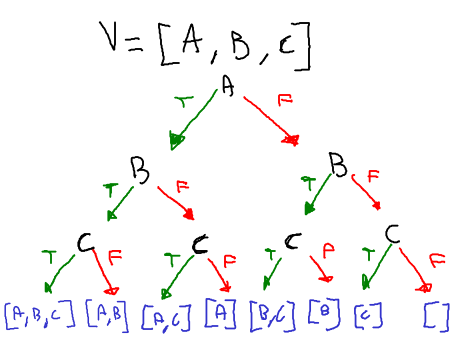
\includegraphics[scale = 0.5]{./img/A1_2.png}
\caption{PowerSet di [a,b,c]} \label{FIG:PowerSet}
\end{figure*}
\subsection{A.2}
Definizione formale di una permutazione (definizione ricorsiva):
\begin{figure*}[!ht]
\centering
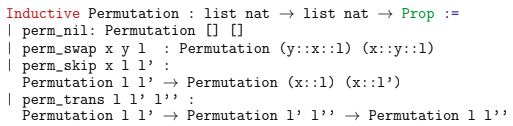
\includegraphics[width=0.7\textwidth]{./img/permutazione_ricorsiva.png}
\caption{Definizione ricorsiva di una permutazione} \label{FIG:recursive_permutation1}
\end{figure*}
\begin{itemize}
	\item perm\_nil: [ ] è permutazione di [ ] (lista vuota è permutazione di se stessa)
	\item perm\_swap: $\forall x,y \in Elements$ e $\forall l \in Lists$ $[y::x::l]$ e $[x::y::l]$ sono una permutazione dell'altra
	\item perm\_skip: dato $x \in Elements$, se $l \in Lists$ è permutazione di $l' \in Lists$ $\Rightarrow [x::l]$ è permutazione di $[x::l']$
	\item perm\_trans: date $l, l', l'' \in Lists$ se $l$ permutazione di $l'$ e $l'$ permutazione di $l'' \Rightarrow l$ è permutazione di $l''$ 
\end{itemize}
\begin{theorem}[Riflessività] $\forall l \in Lists$ Permutation $l$ $l$\end{theorem}
\textit{Dimostrazione}:
\begin{adjustwidth}{2cm}{}
	\textit{caso base}: $l$ = [ ], vale per definizione grazie a perm\_nil\\
	\textit{caso induttivo}: $l = [h::t]$ con $h \in Lists$ e $t \in ELements$.\\
	Grazie all'ipotesi induttiva si può affermare \textit{Permutation} $t$ $t$ e quindi per perm\_skip \textit{Permutation} $[h::t]$ $[h::t]$. Dato che $l = [h::t]$ abbiamo che \textit{Permutation} $l$ $l$.
\end{adjustwidth}
\begin{theorem}[Simmetria] $\forall l,l' \in Lists$, Permutation $l$ $l'$ $\Rightarrow $ Permutation $l' \; l$\end{theorem}
\begin{dimostrazione}
	Assumo che $l$ sia permutazione di $l'$, ma allora devo poter applicare la definizione di \textit{Permutazione}, i 4 casi di figura~\ref{FIG:recursive_permutation1} 


	\textit{primo caso}: $l=[] \; l'=[]$, la proprietà \emph{perm\_nil} ci garantisce sia che $P \;l \; l'$ che $P \; l'\; l$. $l'$ ed $l$ si sono "scambiate"


	\textit{secondo caso}: $l = x::y::t$, $l'= y::x::t$. Assunta vera $P \; l \, l'$, cioè $P \; x::y::t \; y::x::t$, grazie a \emph{perm\_swap} si può affermare $P \; y::x::t \; x::y::t$, cioè $P \; l' \; l$

	\textit{terzo caso}: caso induttivo, è stata applicata \textit{perm\_skip} all'ipotesi quindi $l = x::t$ e $l' = x::t'$ e per definizione $P \; t \, t'$.
	Ma per ipotesi induttiva $P \; t \, t' \Rightarrow P \; t' \, t'$, riapplicando \textit{perm\_skip} ottengo $P \; x::t' \; x::t$ che è esattamente $P \; l' \, l$

	\textit{quarto caso}: caso induttivo, è stata applicata \textit{perm\_trans} all'ipotesi e quindi deve esistere una lista intermedia $l''$ t.c. $P\; l\, l''$ e $P \; l''\, l'$ sono vere.
	Applicando l' ipotesi induttiva alle due affermazioni precedenti otteniamo:$P\; l''\, l$ e $P \; l'\, l''$.\\
	Applicando \textit{perm\_trans} ad entrambe si ottiene $P \; l' \, l$
\end{dimostrazione}
\subsection{A.3}
Dimostrare che è algoritmo che genera permutazioni di una lista di elementi è completo significa dimostrare che genera $n!$ permutazioni, con $n$ pari al numero di elementi. Formalmente:
\begin{theorem}[Completezza] $\forall l \in Lists$, $len($\textit{permutation} $l) = len(l)!$\end{theorem}
\begin{dimostrazione}
	\textit{caso base}: $l$ = [ ]\\
	In questo caso $len(l)! = 0! = 1$.\\
	Allo stesso modo $len(permutation)$ [ ] $= len($[ [ ] ]$) = 1$.\\
	Quindi $len($\textit{permutation} $l) = len(l)!$
	
	\textit{Caso induttivo}: riprendiamo l'ipotesi induttiva: $len(permutation \; t) = len(t)!$
	$l = h::t$, l'enunciato da dimostrare è $$len(permutation \; [h::t]) = len([h::t])!$$
	Risulta ovvio che $len(h::t) = 1 + len(t)$.
	Per ipotesi induttiva il numero di liste generate da $permutation \; t$ sarà $len(t)!$.\\
	Per definizione \textbf{permutation h::t} calcola tutte le permutazioni di $t$ e poi applica ad ogni lista $l' \in permutation \;t$ l'operazione distribute incrementandole di un elemento.
	$$len(h::t) = len(concat\_map \; (distribute \; h) (permutation \; t))$$
\begin{figure*}[!ht]
\centering
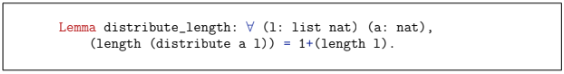
\includegraphics[width=1\textwidth]{./img/A3_distribute.png}
\caption{Lemma distribute lenght} \label{FIG:A3_distribute}
\end{figure*}\\
	Intuitivamente stiamo ripetendo l'operazione $distribute \; h \; l'$ per $len(t) ! $ volte ogni volta producendo una lista di $1 + len(l')$ elementi, quindi otterremo una lista di liste con $(1 + len(l')) * len(t)! $ elementi.\\
	Essendo le liste $l'$ permutazioni di $t$ dovrà valere la sequente equivalenza $len(l') = len(t) $, dato che sto solo eseguendo scambi, non sto aggiungendo ne togliendo elementi.\\
	Sostituendo $len(t)$ a $len(l')$ nell'equazione che specificava il numero di elementi delle liste otteniamo che $permutation  \; h::t$ genera una lista di liste di $(1+len(t)) * len(t)!$ elementi.\\
	Dato che $(1+len(t)) * len(t)! = len([h::t])!$ possiamo affermare che: %perchè è vera l'equivalenza? scemo, è un fattoriale (1 +n)* n! = (1 + n)! per definizione.
	$$len(permutation \; [h::t]) = len([h::t])!$$
\end{dimostrazione}
Notiamo due cose:
Ho affermato che intuitivamente $distribute \; h \; l'$ ripetuto $len(t)$ volte produce una lista di $ 1 + len(l')$ elementi, questo andrebbe dimostrato.
L'altra affermazione che andrebbe dimostrata è "essendo le liste $l'$ permutazioni di $t$".Infatti tale affermazione si basa sull'assunto che \textbf{permutation t} produca permutazioni di $t$, che non è nient'altro che il teorema di corretteza delle permutazioni.
Quindi la completezza si basa sulla correttezza
\subsection{A.4}
\begin{itemize}
	\item \textbf{Permutazioni}:Si può individuare una \emph{risposta} al problema \textbf{Valutazione} generando l'albero di tutte le possibili permutazioni:
		\begin{center}	\scalebox{0.8}{\Tree [  [ [ .1 [  [ .2 [.3 4 ] [.4 3 ] ] [ .3 [.2 4 ] [ .4 2 ] ] [ .4 [ .2 3 ] [ .3 2 ] ] ] ] [ .2 [ [ .1 [ .3 4 ] [ .4 3 ] ] [ .3 [ .1 4 ] [ .4 1 ] ] [ .4 [ .1 3 ] [ .3 1 ] ] ] ] [ .3 [ [ .1 [ .2 4 ] [ .4 2 ] ] [ .2 [ .1 4 ] [ .4 1 ] ] [ .4 [ .1 2 ] [ .2 1 ] ] ] ] [ .4 [ [ .1 [ .3 2 ] [ .2 3 ] ] [ .3 [ .1 2 ] [ .2 1 ] ] [ .2 [ .1 3 ] [ .3 1 ] ] ] ] ] ]}
		\end{center}
		In questo albero un ramo individua una permutazione dell'insieme di partenza, di conseguenza basta percorrerlo calcolando di volta in volta il voto massimo finchè questi non supera il valore fissato (in questa istanza 9).Si ottiene quindi una soluzione, data dalla sequenza di "voti" ottenuta partendo dalla radice e percorrendo il ramo corrispondente fino al padre del nodo che causa il superamento del voto massimo.
		Eseguendo questa operazione su tutti i rami dell'albero si ottengono tutte le \emph{soluzioni}, scegliendo le soluzioni con votazione migliore si ottengono una o più \emph{risposte}.
	\item \textbf{Sottoinsiemi}:Si può individuare una \emph{risposta} al problema \textbf{Valutazione} generando l'albero di tutte le possibili scelte:
		\begin{center}
			\begin{forest}
				for tree={ l sep=20pt, s sep=20pt}
			[1 [2, edge label = {node[midway,left,green] {T}} [3, edge label = {node[midway,left,green] {T}}[4, edge label = {node[midway,left,green] {T}}] [4, edge label = {node[midway,right,red] {F}}]] [3, edge label = {node[midway,right,red] {F}}[4, edge label = {node[midway,left,green] {T}}] [4, edge label = {node[midway,right,red] {F}}]]][2, edge label = {node[midway,right,red] {F}} [3, edge label = {node[midway,left,green] {T}}[4, edge label = {node[midway,left,green] {T}}] [4, edge label = {node[midway,right,red] {F}}]] [3, edge label = {node[midway,right,red] {F}}[4, edge label = {node[midway,left,green] {T}}] [4, edge label = {node[midway,right,red] {F}}]]]] 			\end{forest}
		\end{center}
		A seconda che si scelga un ramo o l'altro la domanda sarà inclusa nella possibile \emph{soluzione} quindi percorrendo un ramo fino alla foglia si giunge sempre ad una sequenza di voti.
		Non tutti i sottoinsiemi così generati sono però \emph{soluzioni}, in quanto alcuni superano il vincolo del voto massimo ammesso (in questo caso 9); considerando solo le \emph{soluzioni} e scegliendo quelle aventi la migliore votazioni si ottengono una o più \emph{risposte}
\end{itemize}
\section{Backtrack}
\subsection{B.1}
Il \textbf{Backtracking} è una tecnica algoritmica atta a migliorare la visita \textbf{Bruteforce} tramite l'elimnazione di alcuni sotto-alberi dell' albero delle scelte che non vale la pena di analizzare.
Più precisamente vengono introdotti due concetti:
\begin{itemize}
	\item \textit{funzione bound:} una funzione che dato un nodo dell'albero delle scelte fornisce un criterio di valutazione sulla possibilità che il sotto-albero avente come radice quel nodo possa o meno fornire una \textit{risposta}
	\item \textit{pruning}: Rimozione di sotto-alberi dall'analisi dell'albero delle scelte per il quale la \textit{funzione bound} predice l'impossibilità di generare \textit{risposte}.Perchè violerebbero i vincoli espliciti o perchè produrrebbero una \textit{soluzione} peggiore di altre trovate in precedenza
\end{itemize}
Il \textbf{Backtracking} può essere visto quindi come una visita \textbf{BruteForce} con k'aggiunta di un filtro.$BT = BF + \text{ \textit{funzione criterio/bound} }+ pruning$
Ogni algoritmo di \textbf{Backtracking} sarà quindi così composto:
\begin{lstlisting}[numbers=left,firstnumber=1,stepnumber=1, xleftmargin=15pt, language=Matlab ]
BT(a,soluzione)=
    completa= completa(a,soluzione)
    if !completa
        rifiuta=rifiuta(a,soluzione)
	if !rifiuta
	    soluzioni = espande(a)
	    foreach soluzione in soluzioni
	        BT(a,soluzione)
    else
    	accetta = accetta(a,soluzione)
        if accetta
	    risposta = soluzione
\end{lstlisting}
\begin{itemize}
	\item \imp{completa(a,soluzione)} (riga 2) è una funzione che resituisce \textit{True} se il cammino dalla radice al nodo attuale può costituire una soluzione.
	\item \imp{rifiuta(a,soluzione)} (riga 4) è una funzione che resituisce \textit{True} se il nodo genera un sotto-albero che non porterà sicuramente ad una risposta, perchè viola un vincolo esplicito o perchè genererebbe una soluzione peggiore di una soluzione trovata in precedenza
	\item \imp{accetta(a,soluzione)} (riga 10) è una funzione che resituisce \textit{True} se la soluzione passata come parametro è migliore dell' attuale \textit{risposta} (e quindi può prenderne il posto)
	\item \imp{espande(a)}(riga 6) è una funzione che espande il nodo, inserendo i suoi figli tra le possibili soluzioni da visitare e da analizzare. La funzione di \textbf{Backtracking} sarà quindi chiamata ricorsivamente su tutte queste possibili soluzioni.
	\item \imp{BT(a,soluzione)} (riga 8): lo scopo di effettuare la chiamata ricorsiva sulle soluzioni appena generate è quello di poter effettuare \textit{pruning} su più sottoalberi possibile, individuando più rapidamente i sottoalberi che contengono \textit{risposte}
\end{itemize}
\subsection{B.2}
\begin{itemize}
	\item \textbf{ordinamento}: una possibile funzione di bound è $a[j-2] > a[j-1]$, presupponendo un vettore $a_0, ... , a_n$ l'algoritmo si basa sul mantenere un indice $j$ t.c. $a_0 \leq ... \leq a_{j-2}$ mentre gli elementi $a_{j}, ..., a_{n}$ non sono ancora stati analizzati.
	Notiamo però che non ha molto senso utilizzare tecniche \textbf{BruteForce} o derivate, perchè l'operazione di confronto fra due numeri può essere sempre effettuata con consto minimo.Potendo confrontare ogni elemento con tutti gli altri elementi posso cancellare una grossa parte dello spazio delle soluzioni.
	L'esempio più sciocco di questa cosa è il \textbf{Boublesort} che , pur confrontando ogni elemento dell'insieme con tutti gli altri, è più efficiente di un approccio \textbf{BruteForce}
	\item \textbf{Cammino Hamiltoniano}: formalmente possiamo definire un cammino Hamiltoniano di un grafo $G$ come una sequenza di archi $SE \subset E, G= (V,E)$ che permette di visitare ogni nodo $V$ esattamente una volta.
	La prima cosa che si può notare è che in questo caso una soluzione equivale ad una risposta, una volta trovato il primo cammino si può effettuare \textit{pruning} di tutto il restante spazio degli stati.\\
	Una buona \textit{funzione bound} è una funzione che interrompe l'esplorazione quando si cerca di inserire un arco non esistente.partendo da un nodo qualsiasi e scegliendo di visitare un altro nodo possiamo sicuramente escludere tutti i nodi che non sono collegati al nodo di partenza da alcun arco, stessa cosa iterando sul prossimo nodo.Bisogna prestare attenzione al fatto che per come è costruito lo spazio degli stati non è possibile visitare un nodo "già visitato".
	\item \textbf{Colorazione di un grafo}: Lo scopo del problema è assegnare un colore $c \in C$ ad ogni nodo $v \in V$ di un grafo $G=(V,E)$. in modo che vertici adiacenti abbiano colore diverso.\\
	Supponiamo di aver colorato fino al nodo $j$ e di avergli dato il colore $c_a$.
	Guardando il corrispettivo stato nella raffigurazione ad albero dello spazio degli stati (Figura~\ref{FIG:B2_colorazione}) i suoi figli saranno tutti i possibili colori di un altro nodo $x$.Se scelgo di scendere lungo il ramo contrassegnato dal colore $c_a$ mi devo assicurare che tra il nodo $j$ ed il nodo $x$ non vi sia alcun arco.\\
Se scelgo di scendere verso uno stato contrassegnato da un colore diverso da $c_a$ posso non fare questo controllo.\\
In entrambi i casi però devo controllare che tutti i nodi connessi da un arco a $x$ abbiano un colore diverso dal colore assegnatogli.\\
\begin{figure*}[!ht]
\centering
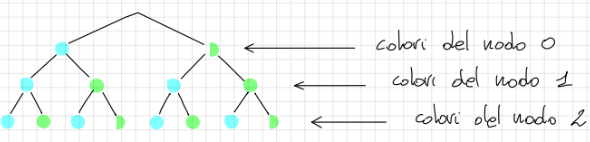
\includegraphics[width=1\textwidth]{./img/B2_colorazione.png}
\caption{Albero delle scelte per colorazione} \label{FIG:B2_colorazione}
\end{figure*}\\

	\item \textbf{Subsetsum}: Siano dati un insieme numerico finito $X$ ed un numero $S$. Determinare l’esistenza di un sottoinsieme $Y$ di $X$, tale che la somma di tutti gli elementi di $Y$ sia pari ad $S$.
		In questo caso la \textit{funzione bound} si basa su tre concetti:
	\begin{enumerate}
		\item se ho trovato una \textit{soluzione} smetto di cercare, sto cercando un generico sottoinsieme, non ho altri vincoli
		\item se la somma degli elementi inseriti nella \textit{potenziale soluzione} $Z$ (la soluzione in fase di costruzione) è maggiore di S non proseguo.
		\item se i primi due punti non sono veri sommo agli elementi presenti nella mia \textit{potenziale soluzione} $Z$ tutti gli altri elementi dell'insieme $X$, se il risultato è comunque minore di $S$ non ha senso proseguire.Anche inserendo tutti gli elementi rimasti non otterrei comunque $S$
	\end{enumerate}
\end{itemize}
ESPANDERE CON ESEMPI???
%pensarci in futuro
\subsection{B.3}
\begin{figure*}[!ht]
\centering
\makebox[\textwidth][c]{
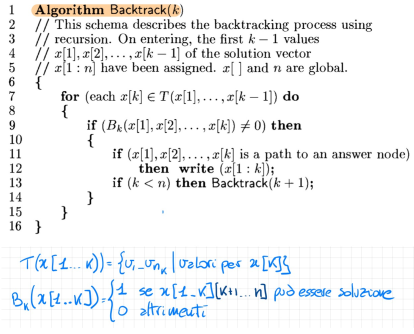
\includegraphics[width=0.85\textwidth]{./img/B3_recursive.png}
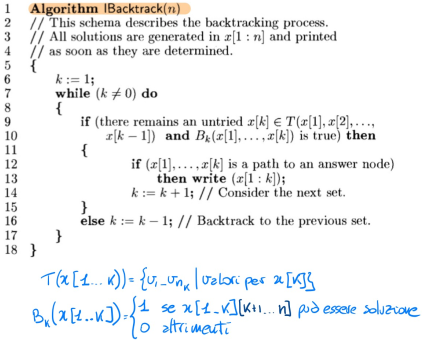
\includegraphics[width=0.85\textwidth]{./img/B3_iterative.png}}
\caption{Backtracking ricorsivo ed iterativo} \label{FIG:B3_algorithms}
\end{figure*}
La sostanziale differenza tra i due algoritmi sta in come viene generato lo \textit{spazio degli stati}, in un caso ricorsivamente, nell'altro tramite un algoritmo iterativo.\\
Questa distinzione è importante in quanto la versione ricorsiva fornisce uno stack implicito, assente nella versione iterativa.Bisogna quindi implementare una struttura dati che permetta di effettuare le operazioni che nel libro (riga 9-10) vengono definite in maniera informale.

Preso $(x_1,x_2,....x_i)$ path dalla radice ad un nodo dell'albero rappresentante lo spazio degli stati definiamo la \textit{funzine bound} $B_k$ come la funzione che restituisce falso quando il path anche se esteso non raggiungerà mai una \textit{soluzione}.\\
$T(x_1,...x_i)$ è il set di tutti i possibili valori di $x_{i+1}$ tali che $(x_1,...x_{i+1})$ è ancora uno stato da analizzare (non è una soluzione).Quindi $T(x-1,...,x_n) = \empty$
\begin{itemize}
	\item \textbf{Algoritmo ricorsivo}:
		Il vettore delle soluzioni $(x_1, ... , x_n)$ è gestito come un array globale $x[1:n]$, $x[1:k]$ contiene tutti gli elementi "accettati", corrisponde alla vettore in corso d'opera che potrebbe portarci ad una \textit{soluzione}.\\
		L'algoritmo prova ad inserire gli elementi rimanenti in k-esima posizione, se il vettore soluzione $(x_1,...,x_k)$ soddisfa $B_k$ si controllo se è una soluzione (riga 11) e la si "stampa", se non lo viene invocata la funzione \textit{Backtrack} ricorsivamente sul nuovo vettore "in costruzione".\\
		Se sono stati inseriti tutti gli elementi e non si è arrivati ad una soluzione (riga 13 $k=n$) bisogna cambiare l'ultimo elemento (figurativamente è come essere al penultimo livello dell'albero e sceglire una foglia sbagliata).
	\item \textbf{Algoritmo iterativo}:\\
		Non avendo uno stack implicito bisogna mantenere un vettore $T$ che contenga tutti i possibili valori che possono essere componenti della soluzione.
		All'inizializzazione $T()$ contiene tutti i possibili valori che è possibile posizionare come primo elemento.\\
		Si tiene conto di quali valori sono stati tentati e quali no, se un valore che non è stato ancora provato soddisfa $B_k$ viene inserito in $T$ (riga 9-10), se il nuovo vettore $T$ è una soluzione viene "stampato" altrimenti si procede nella ricerca come nel caso precedente.\\
		Si noti che questa non è una visita in ampiezza, si sta comunque scendendo su un solo ramo, quiando tutti i valori che potrebbero stare in $x_k$ sono stati tentati e nessuno di loro ha portato a soluzioni k viene decrementato "tornando indietro" e modificando il valore dell'elemento precedente.
\end{itemize}
\section{Branch\&Bound}
\subsection{C.1}
\label{SEC:C_1}
\begin{itemize}
	\item \textcolor{gray}{\textit{dead node}}: radice di sotto-alberi che non sono più espandibili, perchè completi o a causa del pruning
		\item \textcolor{red}{\textit{live node}}: nodo "vivo", cioè alcuni dei suoi figli sono ancora da espandere
		\item \textcolor{red}{\textit{E-node}}: L' \textit{expanded node} è il nodo che si sta visitando in questo momento, cioè il nodo del quale si sta per generare un figlio.L' \textit{E-node} e per definizione un \textit{live node}.
\end{itemize}
A seconda di come si gestisce la visita dei nodi e l'assegnamento dell' \textit{E-node} si può generare una visita dello spazio degli stati differente.
\begin{figure*}[!ht]
\centering
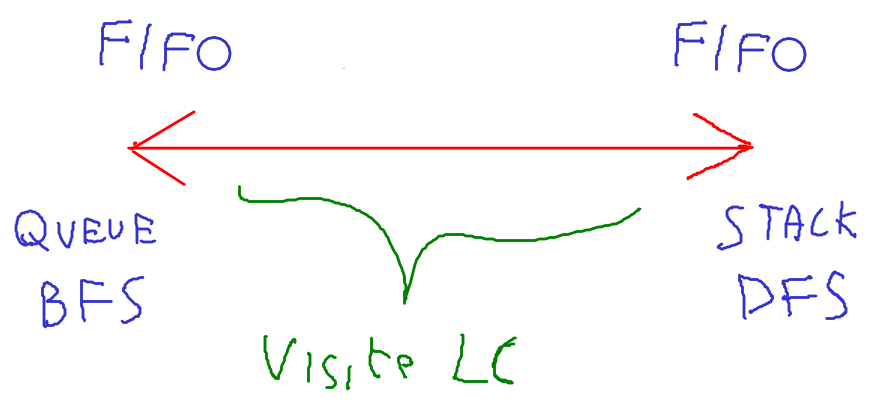
\includegraphics[width=0.7\textwidth]{./img/C_1.png}
\caption{criteri di scelta} \label{FIG:C_1}
\end{figure*}\\
Come mostrato in figura~\ref{FIG:C_1} FIFO e LIFO sono "i due estremi di un ventaglio di possibili criteri di scelta".
Gestendo i live node com uno \emph{stack} e quindi andando ad estrarre l'ultimo nodo inserito si ottiene una visita \textit{depth-first} in cui si trasferisce la condizione di essere \textit{E-node} dal padre al figlio appena generato.
In tal modo un nodo non diventa "\emph{dead} finchè tutti i suoi figli non sono stati visitati, di conseguenza si tende ad arrivare al fondo dell'albero degli stati il più in fretta possibile.
\begin{figure*}[!ht]
\centering
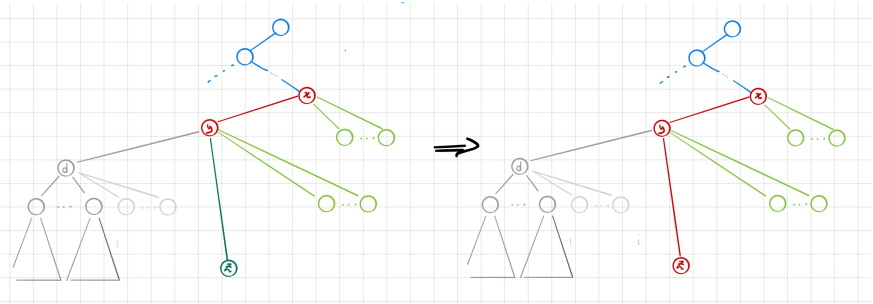
\includegraphics[width=1\textwidth]{./img/C_1_DFS.png}
\caption{visita in profondità} \label{FIG:C_1_DFS}
\end{figure*}\\
In maniera diametralmente opposta funziona la gestione dei nodi con una \emph{queue} in cui il primo nodo inserito è il primo ad essere estratto.Questa politica genera una visita \textit{breadth-first} in cui prima di passare ai nodi del livello successivo i nodi del livello attuale vengono tutti visitati, una volta generati tutti i figli di un nodo questi diventa "dead".
Ciò porta a visite dello spazio degli stati che prima di giungere alle foglie dell'albero degli stati "esplorano" tutte le possibilità.
\begin{figure*}[!ht]
\centering
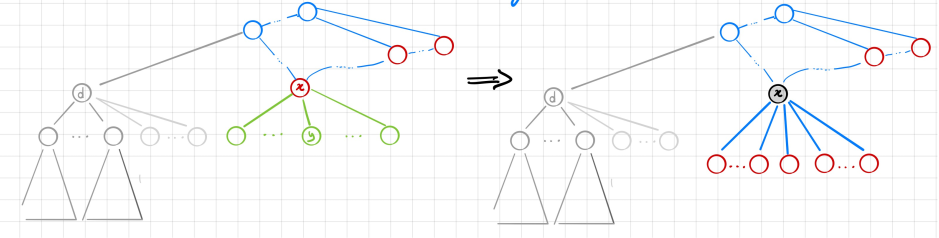
\includegraphics[width=1\textwidth]{./img/C_1_BFS.png}
\caption{visita in ampiezza} \label{FIG:C_1_BFS}
\end{figure*}\\
Come anticipato in figura~\ref{FIG:C_1}, tra DFS e BFS si trovano tutte le possibili politiche intermedie, tra cui le \textit{least cost}. Naturalmente l'individuazione di una politica \textit{least cost} è fortemente dipendente dal problema.
\subsection{C.2}
\begin{figure*}[!ht]
\centering
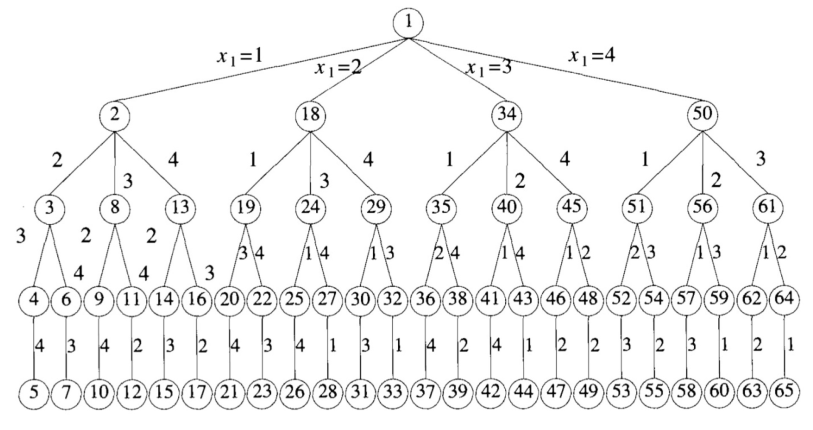
\includegraphics[width=1\textwidth]{./img/C_2.png}
\caption{spazio degli stati 4 regine} \label{FIG:C_2}
\end{figure*}
\textbf{Punto 1}: Presupponiamo di visitare l'albero degli stati tramite le due diverse politiche, effettuando pruning quando necessario.
\begin{itemize}
	\item \textbf{DFS}: La DFS cerca di giungere il prima possibile ad una soluzione, quindi come mostrato in figura~\ref{FIG:C_2_DFS} si scende lungo il ramo più "a sinistra" finchè non si incontra una violazione dei vincoli che induce il pruning (nel nodo 3 ad esempio abbiamo regine in A4 e B3, sulla stessa diagonale).
		Il lato negativo è che spesso la visita in profondità si "infila" in cammini che non portano ad una soluzione, come tutto il sottoalbero generato dalla regina in posizione 2 (A4), potrebbe sembrare conveniente visitare più opzioni possibile in modo da eliminare i cammini che non producono soluzioni il prima possibile.
\begin{figure*}[!ht]
\centering
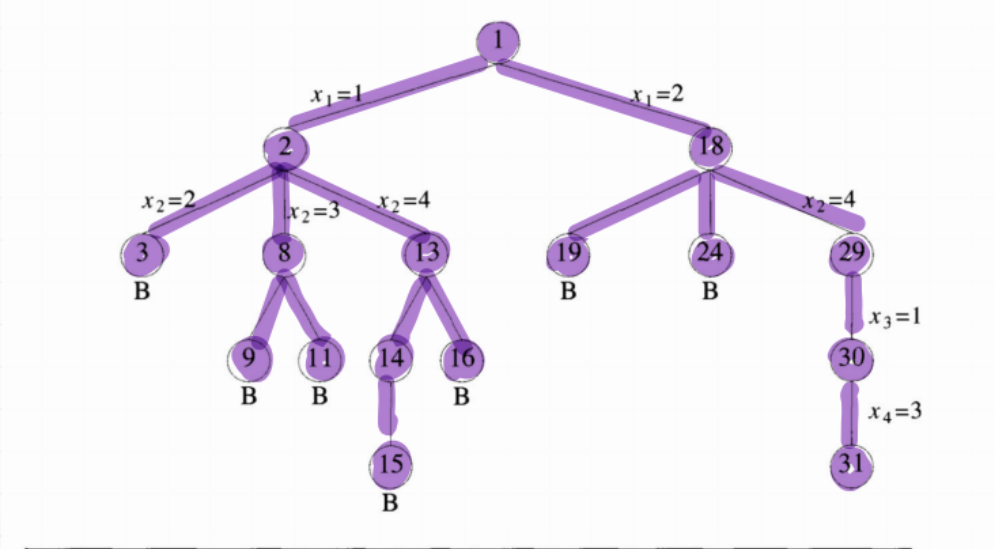
\includegraphics[width=1\textwidth]{./img/C_2_DFS.png}
\caption{Soluzione con DFS} \label{FIG:C_2_DFS}
\end{figure*}\\
	\item \textbf{BFS}:Tramite la visita in ampiezza invece si va ad espandere ogni nodo di un livello dell'albero prima di passare al livello successivo.
		In generale la politica \textit{FIFO} butta via in un sol colpo un sacco di non soluzioni, ma in questo caso prima di incontrare una violazione di qualche vincolo bisogna scendere fino al secondo livello dell'albero, analizzando 16 nodi (che è esattamente il numero di nodi necessari a trovare la \textbf{risposta} con la visita in profondità).
		La politica \textit{LIFO} si dimostra quindi molto meno vantaggiosa, oltretutto si porta dietro un altro svantaggio: se infatti la \textit{FIFO} approfittava dello stack generato dalla ricorsione per mantenere i suoi progressi in memoria nella \textit{LIFO} bisogna costruire una struttura dati atta a mantenere i nodi della "frontiera" in memoria, dato che ogni soluzione viene costruita in parallelo.
		\begin{figure*}[!ht]
\centering
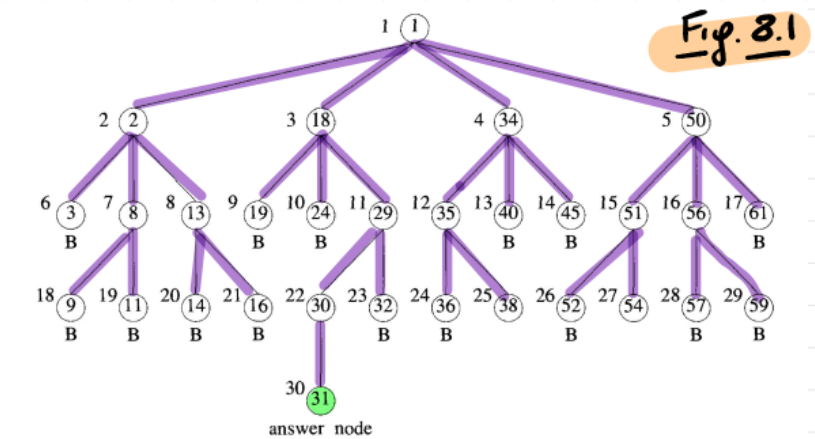
\includegraphics[width=1\textwidth]{./img/C_2_BFS.png}
\caption{Soluzione con BFS} \label{FIG:C_2_BFS}
\end{figure*}
\end{itemize}
\textbf{Punto 2}:
\begin{adjustwidth}{.8cm}{0cm}
	Confrontando le due immagini presenti in figura~\ref{FIG:C_2_DFSvsBFS} notiamo chiaramente che la visita \textit{DFS} è più vantaggiosa in questo caso, giungendo alla soluzione in 16 passi rispetto ai 29 della visita \textit{BFS}.\\
\begin{figure*}[!ht]
\centering
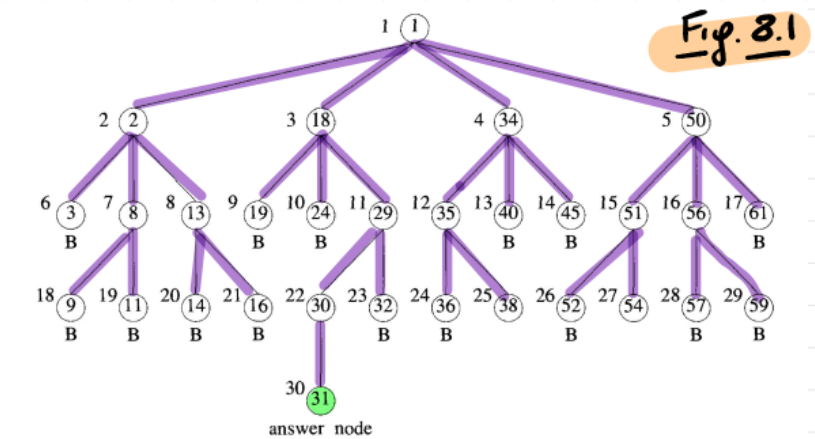
\includegraphics[width=0.49\textwidth]{./img/C_2_BFS.png}
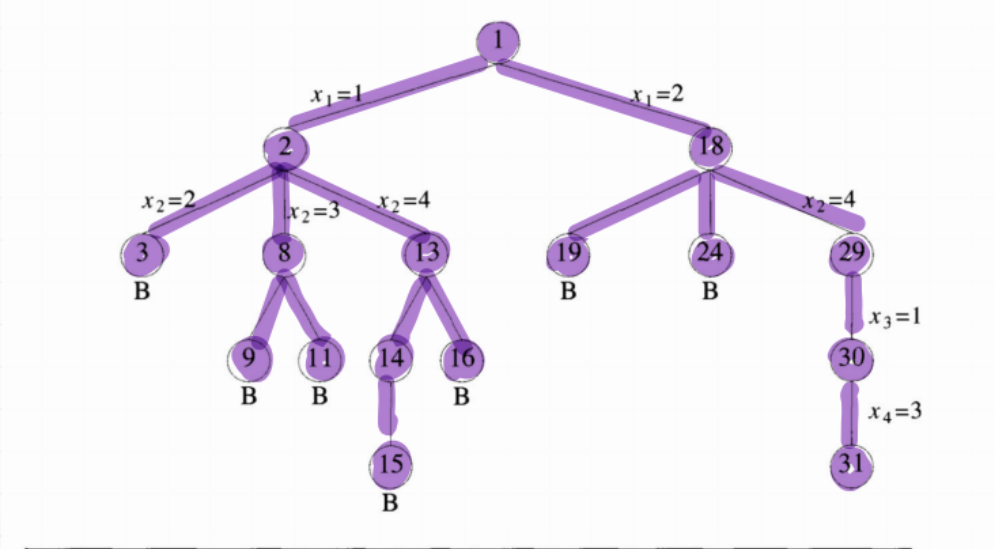
\includegraphics[width=0.49\textwidth]{./img/C_2_DFS.png}
\caption{confronto visita in profondità ed ampiezza} \label{FIG:C_2_DFSvsBFS}
\end{figure*}\\ 
In generale è vero che la politica \textit{FIFO} permette di "buttare via" in un sol colpo un sacco di non soluzioni, ma in questo caso prima di giungere a nodi non accettabili si è obbligati a visitare gran parte dell'albero degli stati.
Sto sì eliminando moltissimi sotto-alberi rispetto alla \textit{DFS} ma per farlo ne sto esplorando molti di più.Più l'albero è ampio rispetto alla sua profondità peggiori sono le prestazioni di una visita in \textit{ampiezza}

%non mi piace proprio questa risposta.


L'ideale sarebbe visitare in ampiezza ma scendere in profondità quando un ramo sembra promettente, per individuare i rami più promettenti si potrebbe ad esempio ordinare i live node minimizzando una delle seguenti proprietà:
\begin{enumerate}
	\item Il numero di nodi nel sottoalbero di $x$ da generare prima di ottenere una \emph{soluzione}.
	\item il numero di livelli che separano il live node dalla risposta.
\end{enumerate}
Il problema derivante dal tentare questo approccio sta proprio nel calcolare le due misure.
Non conoscendo le \textit{soluzioni}, e di conseguenza nemmeno la \textit{risposta}, l'unico modo di effettuare le misure descritte sopra sarebbe quello di esplorare lo spazio degli stati fino ad una \textit{risposta}.
Questa situazione è però paradossale, se conoscessi la risposta non la starei cercando, quindi la misurazione delle due proprietà non è un criterio di ranking applicabile.
\end{adjustwidth}
\subsection{C.3}
\label{SEC:C3}
\textbf{Punto 1}
\begin{adjustwidth}{.8cm}{0cm}
\begin{definition}
	La \textit{funzione costo} $\hat c(x)$ di un \textit{live node x} è: $$\hat c(x) = f(h(x)) + \hat g(x)$$
\end{definition}
\begin{itemize}
	\item$h$ è una funzione che quantifica il lavoro, quindi $h(x)$ è il lavoro noto svolto fin'ora per arrivare al nodo $x$
	\item$f$ è la funzione \emph{peso} monotona, dato in input il lavoro ottenuto da $h$ fornisce un valore proporzionale ad esso utilizzabile come \emph{peso}
	\item$\hat g$ è una \textit{stima} della funzione non nota $g$.Essendo impraticabile calcolare il valore effettivo $g(x)$, $\hat g(x)$ fornisce una stima di quello che sarà il costo della costruzione di un cammino dal nodo $x$ fino ad una eventuale \textit{risposta} che il sotto-albero di radice $x$ contiene.\\
		la funzione $\hat g$ non è generalizzabile, dipende dal problema.
\end{itemize}
E' necessario introdurre una funzione costo in quanto non è possible calcolare accuratamente il \textit{ranking} di un nodo, bisogna quindi ripiegare su una stima che permetta scegliere in maniera intelligente il prossimo \textit{E-node}.
E' composta principalmente da due parti, il \textit{costo noto} ed il \textit{costo stimato}\\
\begin{figure*}[!ht]
\centering
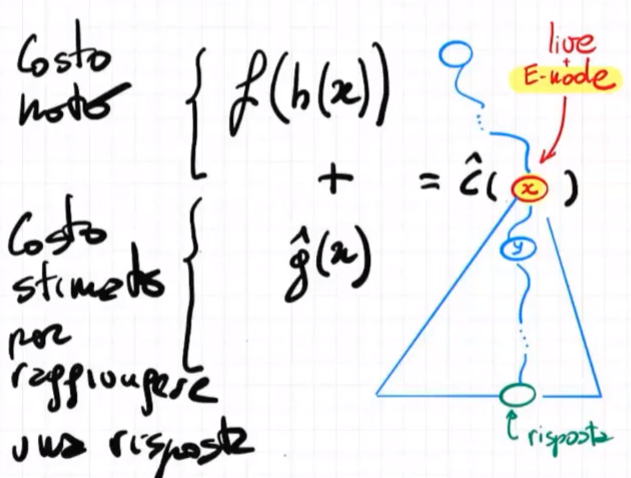
\includegraphics[width=0.4\textwidth]{./img/C_3_punto1.png}
\caption{funzione costo} \label{FIG:C_3_punto1}
\end{figure*}\\
Notiamo anche che dati due nodi $x,y$ se $y$ è un discendente di $x$ ci aspettiamo che la funzione $\hat g(x) > \hat g(y)$, altrimenti la funzione costo è mal formata.
\end{adjustwidth}
\textbf{punto 2}
\begin{adjustwidth}{.8cm}{0cm}
DOPO AVER RICORDATO? cioè devo riscrivere la definizione? mi sembra ridondante.\\
%copia ed incolla magari abbreviando la definizione
Analizziamo la situazione: $f(h(x)) =0$, in questo caso il \textit{costo noto} non ha influenza sul risultato generato da $\hat c(x)$ e la \textit{funzione costo} può essere riscritta come $$\hat c(x) = \hat g(x)$$
Questo ci riporta ad un algoritmo di \textit{Backtracking}, in quanto non vi è "penalità" nell' espandere nodi in profondità nell'albero degli stati.Considerando che dati due nodi $x,y$ se $y$ è un discendente di $x$ allora $\hat g(x) > \hat g(y)$ la scelta che minimizza la \textit{funzione costo} è sempre quella che espande un nodo di livello successivo, quindi una \textit{D-search}.
Immaginiamo ad esempio due \textit{live node} $x,z$, l' \textit{E-node} è $x$ e genera due discendenti: $w_1, w_2$.
		\begin{align}
			&0 + \hat g(x) < 0 + \hat g(z) \text{ dato che $x$ è \textit{E-node}} \notag \\
			&0 + \hat g(w_1) \leq 0 + \hat g(w_2) < 0 + \hat g(z) \text{ dato che $\hat g$ è monotona} \notag\\
			&\hat c(w_1) \leq \hat c(w_2) < \hat c(z) \notag
	        \end{align}
		Di conseguenza il prossimo \textit{E-node} sarà scelto tra $w_1$ e $w_2$
\end{adjustwidth}
\textbf{punto 3}
\begin{adjustwidth}{.8cm}{0cm}
DOPO AVER RICORDATO? cioè devo riscrivere la definizione? mi sembra ridondante.\\
%copia ed incolla magari abbreviando la definizione
Analizziamo la situazione: $f(h(x)) \neq 0$, $\hat c(x) = f(h(x)) + \hat g(x)$.\\
Riprendendo l'idea del punto precendente abbiamo due \textit{live node} $x,z$, l'\textit{E-node} è $x$ e genera discendenti chiamati $w_1,..., w_n$.
\begin{align}        
	f(h(x)) + \hat g(x) &< f(h(x)) + \hat g(z) \notag \\
	c(w_1) = (f(h(x) + &\Delta) + (\hat g(x) - \Delta') \notag \\
	c(w_1) = (f(h(x)) + &\hat g(x)) + (\Delta - \Delta') \notag
	\end{align}
	\begin{equation}
	\begin{cases}
		se \; (\Delta - \Delta') &\leq 0 \text{ proseguiamo lungo il ramo di $w_1$} \notag \\
		se \; (\Delta >> \Delta') &\text{ $w_1$ non è un nodo conveniente} \notag
	\end{cases}
	\end{equation}
In questa situazione i valori di $\hat c(w_1), \hat c(w_2), . . . , \hat c(w_n)$ possono superare quelli relativi a live node inseriti nella lista prima di $w_1, w_2, . . . , w_n$ e, quindi, risultare sconvenienti da seguire rispetto ad altri.
\end{adjustwidth}
\subsection{C.4}
\label{SEC:C4}
Come già mostrato in sezione~\ref{SEC:C_1}, più precisamente in figura~\ref{FIG:C_1} \textit{FIFO} e \textit{LIFO} sono "i due estremi di un ventaglio di possibili criteri di scelta" ed in quanto tali possono essere ottenuti tramite una precisa formulazione della \textit{funzione costo}.
Infatti analizzando la \textit{funzione costo} $\hat c(x) = f(h(x)) + \hat g(x)$ si nota facilmente quali sono le possibili casistiche che possono portare ad un estremo o all'altro.
\begin{itemize}
	\item $\hat c(x) = f(h(x)) + 0$ In questo caso la \textit{funzione costo} non subisce l'influenza del \textit{costo stimato}.
		La \textit{funzione costo} può essere riscritta come $$\hat c(x) = f(h(x))$$
		Intuitivamente i \textit{nodi} più vicini alla radice avranno un costo inferiore, di conseguenza verranno scelti per primi e si verificherà la classica situazione caratteristica delle \textit{Breadth-search}: tutti i nodi appartenenti ad un livello dell'albero verranno esaminati prima di procedere con l' espansione dei nodi del livello successivo.
Immaginiamo ad esempio due \textit{live node} $x,z$, l' \textit{E-node} è $x$ e genera due discendenti: $w_1, w_2$.
                \begin{align}
                        &f(h(x)) + 0 < f(h(z)) + 0 \text{ dato che $x$ è \textit{E-node}} \notag \\
                        &f(h(w_1)) + 0 = f(h(w_1)) + 0 > f(h(z)) + 0 \\
                        &\hat c(w_1) = c(w_2) > \hat c(z) \notag
                \end{align}
Di conseguenza il prossimo \textit{E-node} sarà sicuramente $z$.\\
L'equazione del punto (1) deriva dal fatto che per giungere a $w_1,w_2$ è stato fatto del lavoro in più, esattamente il lavoro necessario ad espandere $x$

	\item $\hat c(x) = 0 + \hat g(x)$ Questa casistica, già affrontata nella sezione~\ref{SEC:C3} al \textbf{Punto 2} si riconduce ad una \textit{D-search}.
		Se $f(h(x)) =0$ il \textit{costo noto} non ha influenza sul risultato generato da $\hat c(x)$ e la \textit{funzione costo} può essere riscritta come: $$\hat c(x) = \hat g(x)$$
Questo ci riporta ad un algoritmo di \textit{Backtracking}, in quanto non vi è "penalità" nell' espandere nodi in profondità nell'albero degli stati.
Considerando che dati due nodi $x,y$ se $y$ è un discendente di $x$ allora $\hat g(x) > \hat g(y)$ la scelta che minimizza la \textit{funzione costo} è sempre quella che espande un nodo di livello successivo, quindi una \textit{D-search}.
Immaginiamo ad esempio due \textit{live node} $x,z$, l' \textit{E-node} è $x$ e genera due discendenti: $w_1, w_2$.
                \begin{align}
                        &0 + \hat g(x) < 0 + \hat g(z) \text{ dato che $x$ è \textit{E-node}} \notag \\
                        &0 + \hat g(w_1) \leq 0 + \hat g(w_2) < 0 + \hat g(z) \text{ poichè $\hat g$ è monotona} \notag\\
                        &\hat c(w_1) \leq \hat c(w_2) < \hat c(z) \notag
                \end{align}
Di conseguenza il prossimo \textit{E-node} sarà scelto tra $w_1$ e $w_2$

\end{itemize}
\subsection{C.5}
L'algoritmo in figura~\ref{FIG:C5} rappresenta un generico algoritmo per una visita \textit{Least Cost}.\\
\begin{figure*}[!ht]
\centering
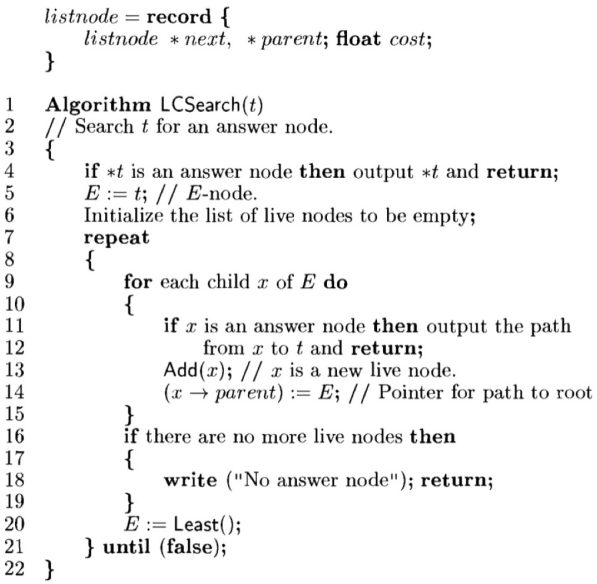
\includegraphics[width=0.8\textwidth]{./img/C5.png}
\caption{Algoritmo Least Cost} \label{FIG:C5}
\end{figure*}\\
La struttura dati su cui si appoggia è una lista di \textit{record}, in cui ogni record può essere visto come un "nodo" dell'albero che rappresenta lo spazio degli stati.\\
La struttura dati \textit{listnode} fornisce due operazioni \texttt{Add(\textit{x})} e \texttt{Least()} che forniscono la possibilità di inserire o estrarre record.
Possiamo assumere che l'operazione \texttt{Least()} estrae dalla struttura dati il nodo che restituisce il minor valore quando inserito come imput nella funzione costo $ \hat c(\cdot)$.
A seconda di come sono è implementata l'operazione \texttt{Add(\textit{x})} avremo differenti comportamenti nel caso si incontrassero nodi aventi lo stesso \textit{costo}, allo stesso modo di quanto discuso in sezione \ref{SEC:C3} e sezione \ref{SEC:C4}.

Analisi dell'algoritmo:
\begin{itemize}
	\item Le righe 4-6 inizializzano la struttura dati ed impostano la radice dell'albero come \imp{E-node}.
	\item In riga 7 viene iniziato un ciclo che si concluderà quando tutto lo spazio degli stati sarà stato completamente esplorato oppure sarà stata individuata una \textit{risposta}, non vi è alcun criterio di \textit{pruning}
	\item Le righe 9-15 sono il cuore della ricerca, vengono generati tutti i figli dell' \imp{E-node}, se nessuno di loro è \textit{risposta} vengono aggiunti alla lista dei \textit{live node} tramite l'operazione \texttt{Add(\textit{x})}. %in realtà viene pure impostato il loro padre ma ciò è irrilevante, dillo a voce
	\item Quando tutti i figli di un nodo sono stati aggiunti alla \textit{listnode} il nodo è sostanzialmente diventato un \textit{Dead node} ed il nodo che fornisce il minimo valore della \textit{funzione costo} viene scelto come prossimo \imp{E-node}.
\end{itemize}
\subsection{C.6}
\label{SEC:C6}
L'idea da cui partire per sviluppare una \textit{funzione costo} per \imp{SubsetSum} è quella di individuare un intervallo di valori al cui interno è compreso il valore \emph{s} del problema \imp{SubsetSum} $X =({X_0 ... X_{n-1}},S)$ 
Per chiarezza presentiamo con $X_k$ il valore numerico di un elemento, $x_k \in {0,1}$ indica se il numero è inserito nell'insieme o no.
Come descritto nella sezione~\ref{SEC:C3} la \textit{funzione costo} $\hat c$ è composta da una \textit{parte nota} ed una \textit{parte stimata}.
$$\hat c(x[0..j)) = f(h(x[0..j))) + \hat g(x[0..j))$$
\begin{itemize}
	\item La parte nota è facilmente individuabile come la somma dei numeri già inseriti nell'insieme.$$ f(h(x[0..j)))=\sum_{0 \leq k < j} X_kx_k$$
	\item La parte stimata viene calcolata in modo che valga la seguente condizione:
		$$ f(h(x[0..j))) + \hat g(x[0..j)) - V \leq S \leq f(h(x[0..j))) + \hat g(x[0..j)) $$
	Rivmuovendo $V$ ottengo una approssimazione per difetto di $S$, se non lo rimuovo ottengo una approssimazione per eccesso.
	Se però $V$ viene preso dall'insieme $X$ diventa l'elemento che se tolto dalla somma degli elementi che mi rimangono da inserire fornisce la migliore approssimazione per difetto/eccesso di $S$
	$ \hat g(x[0..j))=\sum_{j \leq k < split} X_k$ in cui il valore split è t.c:
	$$\sum_{j \leq k < split-1} X_k \leq S \leq \sum_{j \leq k < split} X_k$$
\end{itemize}
Lo scopo di questa funzione costo è esplorare in maniera più intelligente lo spazio delle soluzioni, la strategia \textit{LC} diventa la strategia di scelta del prossimo \textit{E-node} tra tutti i possibili \textit{live-node}.
Ma a parità di \imp{costo} bisogna comunque affidarsi ad uno dei due criteri (\textit{LIFO/FIFO}) ma si potrebbe pensare anche di non affidarsi ad un criterio fisso e decidere randomicamente di volta in volta, per introdurre "perturbazioni" che riducano il rischio di svolgere ripetutamente scelte sbagliate.

E naturalmente anche possibile migliorare l'efficenza di questa visita tramite pruning rimuovendo i rami dell'albero il cui valore $ f(h(x[0..j))) + \hat g(x[0..j)) - V > S$.Non ha infatti senso esplorare i sottoalberi che generano, in quanto non possono contenere soluzioni.
%oltretutto nella funzione costo cerco di minimizzare il lower bound, altrimenti sarebbe un branch and bound
\subsection{C.7}
Per semplicità di comprensione individuiamo la n-esima casella con le sue indicazioni di riga e colonna $n = i*4 + j$, quindi la vediamo come una matrice.

L'algoritmo quando posiziona una regina su una cella incrementa di 1 il valore di tutte le caselle che la regina può "mangiare" quindi tutte le caselle sulla stessa riga, tutte le caselle sulla stessa colonna e le righe sulle due diagonali.
\begin{itemize}
	\item La parte nota è data dal numero di caselle della scacchiera occupabili, quindi le celle in nessuna regina è presente o può muoversi e di conseguenza mangiare.
	\item la stima $\hat g$ è data dalla somma del valore di tutte le caselle adiacenti alla casella che si sta analizzano cambiata di segno.
\end{itemize}
Si può facilmente effettuare pruning, andando a rimuovere i sotto-alberi generati dai nodi che rappresentano l'inserimento di regine su caselle $x \in X$ aventi $x_{ij} \neq 0$.\\
\begin{figure*}[!ht]
\centering
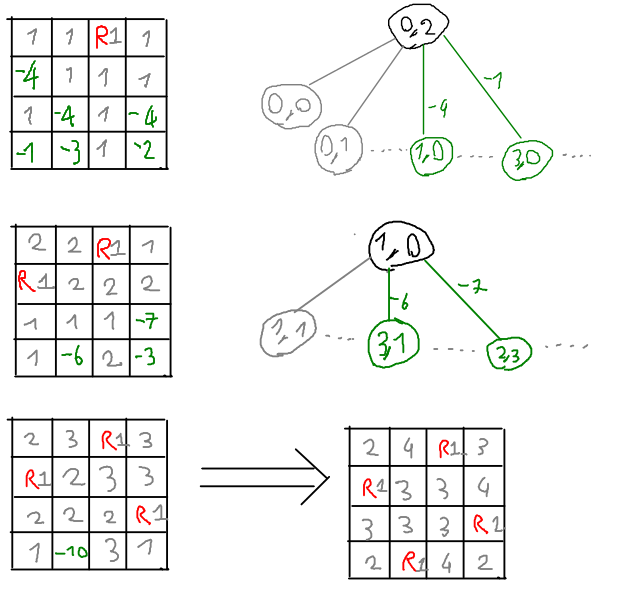
\includegraphics[width=0.8\textwidth]{./img/C7.png}
\caption{Algoritmo Least Cost 4-regine} \label{FIG:C7}
\end{figure*}\\

Formalmente, identifichiamo la cella sulla i-esima riga e j-esima colonna con $x_{i\,j}$ ed chiamiamo $x_{i\,j}^c$ la variabile che indica se la cella è occupata o no.
\begin{equation*}
	x_{i\,j}^c\begin{cases}
		1 \; se \; x_{i\,j} = 0\\
		0 \; se \; x_{i\,j} > 0
	\end{cases}
\end{equation*}
Allora
$$ \hat c(x_{ij})= \sum^n_{i=0} \sum^n_{j=0} x_{i\,j}^c + \sum_{i=i-1}^{i+1} \sum_{j=j-1}^{i+1} x_{i\,j}$$  

Come in sezione \ref{SEC:C6} a parità di \imp{costo} bisogna comunque affidarsi ad uno dei due criteri (\textit{LIFO/FIFO}).
Ad esempio al secondo passo è stato scelto di posizionare la regina nella cella $x_{0 \, 1}$ ma la si sarebbe potuta inserire anche in $x_{1 \, 2}$ o $x_{2 \, 3}$.
Notiamo che se la regina fosse stati inserita in $x_{1 \, 2}$ non avremmo potuto ottenere una soluzione. 
\subsection{C.8}
La qualità di tutti gli algoritmi greedy può essere migliorata ordinando gli elementi in base al rapporto $\frac{valore}{peso}$, operazione con costo $O(n\log_n)$.
In generale le approssimazioni fornite da algoritmi greedy per la risoluzione di \imp{Knapspack} sono molto vicine alla risposta. %il prof se non sbaglio diceva 80%
Per entrambi gli algoritmi presupponiamo tre strutture dati di dimensione $n$, "vettore" $w$ dei pesi, "vettore" $p$ dei profitti e "vettore" $x$ delle scelte. $x[j] \in {0,1}$ indica se l'elemento di indice $j$ è inserito o no nello zaino.
%mi fa schifo il temine vettore, vorrei indicare una generica struttura dati.
\begin{itemize}
	\item \textbf{Greedy}: 
		\begin{lstlisting}[language=Matlab]
	w_tot = 0
	z = 0
	for j = 0 to n do
		if w_tot + w[j] <= c then
			x[j] = 1
			w_tot = w_tot + w[j]
			z = z + p[j]
		else x[j] = 0
		\end{lstlisting}
		L'algoritmo può essere intuitivamente riassunto in 3 passi
		\begin{enumerate}
			\item prova ad inserire un elemento di peso $w[j]$ nello zaino
			\item se l' aggiunta dell' elemento non causa il superamento del limite $c$ inseriscilo, passa al prossimo altrimenti.
			\item analizzati tutti gli elementi concludi.
		\end{enumerate}
	\item \textbf{Greedy-split}:
		\begin{lstlisting}[language=Matlab]
	w_tot = 0
	z = 0
	j = 0
	while w_tot + w[j] <= c
			x[j] = 1
			w_tot = w_tot + w[j]
			z = z + p[j]
			j = j + 1
		\end{lstlisting}
		Questo algoritmo è ancora meno preciso dell' algoritmo \textbf{greedy}, in quanto interrompe la ricerca appena si incontra un elemento che causa il superamento del limite $c$.
		E' però anche più efficiente, non dovendo analizzare altri elementi che rischiano di non poter essere inseriti nello zaino.
		\begin{enumerate}
			\item prova ad inserire un elemento di peso $w[j]$ nello zaino
			\item se l' aggiunta dell' elemento non causa il superamento del limite $c$ inseriscilo, altrimenti concludi la visita.
		\end{enumerate}
\end{itemize}
Entrambi gli algoritmi soffrono di un problema, sono \textit{potenzialmente pessimi}, ma non è questo il caso presentato nella domanda.
$$(\vec w = (1,M)), \vec p = (3,M), 2M$$
Questo caso ha un particolarità, analizzando i pesi si può notare che $p_{max} = M +1$ essendoci solo due elementi, uno di peso $M$ l'altro di peso $1$.La particolarità è che $2M > M + 1 \forall M > 0$, quindi se lo zaino ha una capienza maggiore di $0$ potrà sempre contenere tutti gli elementi che siamo intenzionati ad inserire.
\begin{figure*}[!ht]
\centering
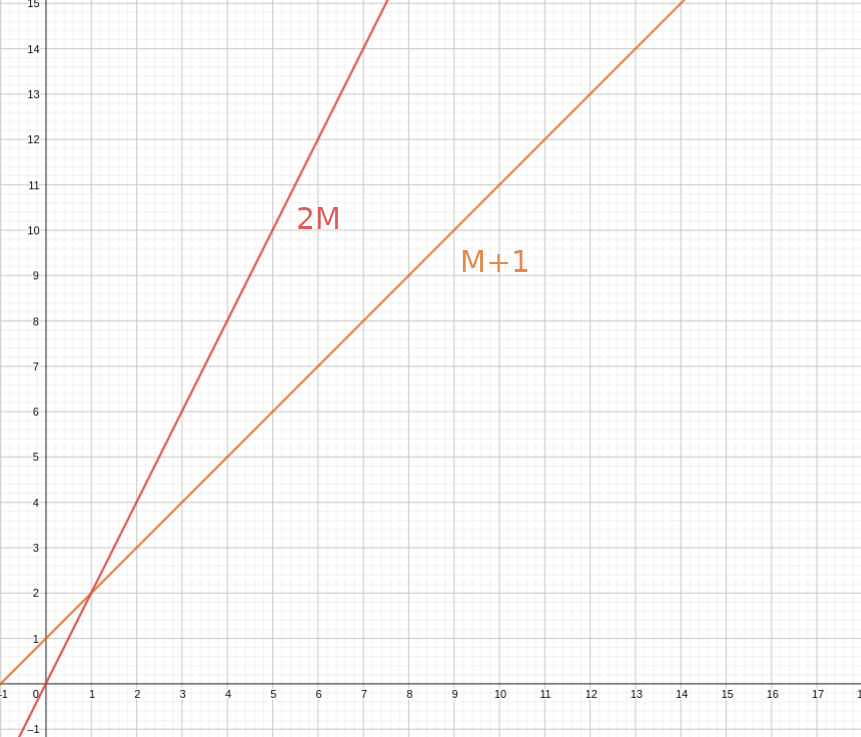
\includegraphics[width=0.5\textwidth]{./img/C_8.png}
\caption{Dimensione soluzione vs spazio al crescere di M} \label{FIG:C_8}
\end{figure*}\\
In questo caso \textbf{Greedy-split} si dimostra perfettamente identico in termini di soluzione a \textbf{Greedy}, in quanto non si incontra mai un elemento che causa il superamento del limite $c$, unica differenza dei due algoritmi.
\subsection{C.9}
La qualità di tutti gli algoritmi greedy può essere migliorata ordinando gli elementi in base al rapporto $\frac{valore}{peso}$, operazione con costo $O(n\log_n)$.
In generale le approssimazioni fornite da algoritmi greedy per la risoluzione di \imp{Knapspack} sono molto vicine alla risposta. %il prof se non sbaglio diceva 80%
Per entrambi gli algoritmi presupponiamo tre strutture dati di dimensione $n$, "vettore" $w$ dei pesi, "vettore" $p$ dei profitti e "vettore" $x$ delle scelte. $x[j] \in {0,1}$ indica se l'elemento di indice $j$ è inserito o no nello zaino.
%mi fa schifo il temine vettore, vorrei indicare una generica struttura dati.
Inoltre supponiamo non esista alcun elemento di indice $j$ tale che $p[j] > c$.
\begin{itemize}
\item \textbf{Greedy-split}:
		\begin{lstlisting}[language=Matlab]
	w_tot = 0
	z = 0
	j = 0
	while w_tot + w[j] <= c
			x[j] = 1
			w_tot = w_tot + w[j]
			z = z + p[j]
			j = j + 1
		\end{lstlisting}
		Questo algoritmo interrompe la ricerca appena si incontra un elemento che causa il superamento del limite $c$.
		\begin{enumerate}
			\item prova ad inserire un elemento di peso $w[j]$ nello zaino
			\item se l' aggiunta dell' elemento non causa il superamento del limite $c$ inseriscilo, altrimenti concludi la visita.
		\end{enumerate}
	Questo algoritmo, come \textbf{Greedy} soffre di un problema, è \textit{potenzialmente pessimo}.\\
	L' istanza di \imp{KP} presentata nella domanda è un esempio di questa situazione:
	$$(\vec w = (1,M), \vec p = (2,M), M)$$
	Infatti ordinando gli elementi per $pw = \frac{profit}{weight}$ notiamo che 
	\begin{align}
		pw_1  &> pw_2 \notag \\
		\frac{2}{1} &> \frac{M}{M} = 1 \notag
	\end{align}
	Seguendo l'algoritmo \textbf{Greedy-split} verrà scelto l'elemento con $pw$ maggiore, cioè l'elemento con indice 1.\\
	Finchè $M \leq p_1$ questo ci fornisce una \textit{risposta} in quanto il scegliendo l'elemento con indice 1 abbiamo un profitto maggiore o uguale di quello che avremmo scegliendo l'elemento con indice 2 (quello con \textit{peso} e \textit{profitto} pari ad $M$.\\
	Quando però $ M > p_1$ l'algoritmo sceglie erroneamente, infatti considerando $M =3$  il profitto ottenuto scegliendo l'elemento di indice 1 è 2, mentre il profitto ottenibile scegliendo il secondo elemento è 3.\\
	Il rapporto $\frac{profitto \; ottenuto}{profitto \; ottimo}$ decresce al crescere di $M$ rendendo sempre più "incorretta" la soluzione offerta da \textbf{Greedy-split}. 
\begin{figure*}[!ht]
\centering
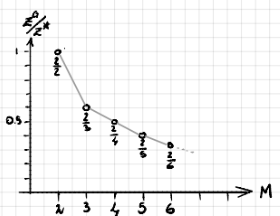
\includegraphics[width=0.5\textwidth]{./img/C_9_greedy.png}
\caption{Qualità della soluzione di \textbf{Ext-Greedy} al crescere di $M$} \label{FIG:C_9_greedy}
\end{figure*}\\
\item \textbf{Ext-Greedy}:
		\begin{lstlisting}[numbers=left,firstnumber=1,language=Matlab, stepnumber=1, xleftmargin=50pt]
w_tot = 0
z=0
for j = 0 to n do
	if w_tot + w[j] <= c then
		x[j] = 1
		w_tot = w_tot + w[j]
		z = z + p[j]
	else x[j] = 0
for j = 0 to n do
	if p[j] > z
		z = p[j]
		for k = 0 to n do x[k] = 0
		x[j] = 1
		\end{lstlisting}
		\begin{enumerate}
			\item prova ad inserire un elemento di peso $w[j]$ nello zaino (riga 4)
			\item se l' aggiunta dell' elemento non causa il superamento del limite $c$ inseriscilo, passa al prossimo altrimenti. (righe 3-8)
			\item analizzati tutti gli elementi concludi il ciclo.
			\item confronta il valore ottenuto dal ciclo con il valore di ogni oggetto, se esiste un elemento che fornisce un risultato migliore di quello trovato nel ciclo (righe 3-8) allora inserisco solo quell'elemento nello zaino. $Z_{risposta} = max\{z, max\{p_1 ... p_n\}\}$
		\end{enumerate}
		Questo algoritmo risolve il problema degli algoritmi \textbf{Greedy} e \textbf{Greedy-split} in qquanto se si verifica una situazione analoga a quella presentata nella domanda $(\vec w = (1,M), \vec p = (2,M), M)$ verrà preso l'elemento avente peso e profitto $M$ in quanto il suo profitto è superiore al profitto offerto dagli elementi inseriti in base all'incremento locale.
\begin{figure*}[!ht]
\centering
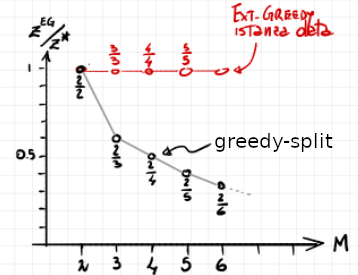
\includegraphics[width=0.5\textwidth]{./img/C_9_ext.png}
\caption{Comportamento \textbf{Ext-Greedy} rispetto a \textbf{Greedy-split}} \label{FIG:C_9_ext}
\end{figure*}\\
\end{itemize}
\subsection{C.10}
\textbf{Ext-Greedy}:
		\begin{lstlisting}[numbers=left,firstnumber=1,language=Matlab, stepnumber=1, xleftmargin=10pt]
w_tot = 0
z=0
for j = 0 to n do
	if w_tot + w[j] <= c then
		x[j] = 1
		w_tot = w_tot + w[j]
		z = z + p[j]
	else x[j] = 0
for j = 0 to n do
	if p[j] > z
		z = p[j]
		for k = 0 to n do x[k] = 0
		x[j] = 1
		\end{lstlisting}
		\begin{enumerate}
			\item prova ad inserire un elemento di peso $w[j]$ nello zaino (riga 4)
			\item se l' aggiunta dell' elemento non causa il superamento del limite $c$ inseriscilo, passa al prossimo altrimenti. (righe 3-8)
			\item analizzati tutti gli elementi concludi il ciclo.
			\item confronta il valore ottenuto dal ciclo con il valore di ogni oggetto, se esiste un elemento che fornisce un risultato migliore di quello trovato nel ciclo (righe 3-8) allora inserisco solo quell'elemento nello zaino. $Z_{risposta} = max\{z, max\{p_1 ... p_n\}\}$
		\end{enumerate}
		\begin{definition}[K-approssimazione]:Un algoritmo $G$ fonisce una \textit{k-approssimazione} con $0 \leq k \leq 1$ se per ogni istanza $I$ del problema $P$ che $G$ risolve , il rapporto tra il profitto calcolato con $G, z^G(I)$ ed il profitto ottimale $z^*_p(I)$ è almeno pari a $k$:
			$$\forall I, \frac{z^G(I)}{z^*_p(I)} \geq k$$
		La k-approximation è tight, stretta, se non è possibile migliorarla.
			$$\exists T, \frac{z^G(T)}{z^*_p(T)}=k$$
\end{definition}
\begin{theorem} Ext-greedy $\in \frac{1}{2}-approximation$ del \textbf{Knapsack problem}
$$\forall I_{kp}, \frac{z^{EG}(I_{kp})}{z^*_p(I_{kp})} \geq \frac{1}{2}$$
\end{theorem}
\begin{dimostrazione}
	La dimostrazione si basa sulla gerarchia dei profitti presentata in sezione~\ref{SEC:C.13}.\\
$$\hat p \leq z^G \leq z^* \leq \lfloor z^LP \rfloor  \leq z^LP \leq \hat p + p_split \leq z^G + p_{split}$$


$\forall I_{kp} \; z^*(I_{kp}) \leq z^G(I_{kp}) + p_{max}$ ove $p_{max}$ è il massimo profitto offerto da un elemento (non è p-split).\\
possiamo maggiorare entrambi i membri dell'equazione:
$$z^G(I_{kp}) \leq max\{z^G(I_{kp}), p_{max}\}$$
$$p_{max} \leq max\{z^G(I_{kp}), p_{max}\}$$
$$ \textit{allora } z^G(I_{kp}) + p_{max} \leq max\{z^G(I_{kp}), p_{max}\} + max\{z^G(I_{kp}), p_{max}\}$$
Notiamo che l'espressione $max\{z^G(I_{kp}), p_{max}\}$ coincide con la definizione di \textbf{Extended-Greedy}, quindi posso sostituirlo nell'equazione.
$$\triangleq z^{EXT_GREEDY}(I_{kp}) + z^{EXT_GREEDY}(I_{kp}) = 2z^{EXT_GREEDY}(I_{kp}) $$

nel caso peggiore il \textit{profitto ottimale} è il doppio del profitto fornito da \textbf{Extended-Greedy}.
%il prof sfasa e dice l'opposto https://unito.webex.com/recordingservice/sites/unito/recording/f80a23c69d61103a9dca005056810dc5/playback (minuto 9:40 circa)
\end{dimostrazione}
\begin{theorem} $\frac{1}{2}$ è una k-approssimazione tight per \textbf{Ext-Greedy}
	$$\nexists K', K' > \frac{1}{2} \; t.c. \; \forall I, \frac{z^{EG}(I)}{z^*_p(I)} \geq K'$$
\end{theorem}
\begin{dimostrazione}
	Per dimostrarlo basta trovare un'istanza $I$ che fornisca un rapporto $K=\frac{1}{2}$.In realtà possiamo identificare un'intera classe.
	$$I= ((\vec w = (1,M,M), \vec p = (Q,M,M),2M) \text{ con } 1<Q<2 \leq M$$
	%io qui ho inserito il \leq M, infatti questa istanza non può esistere con M=1. con M=1 troviamo esattamente Z^*, una 1-approx. il prof ha fatto un errore scrivendo 1<Q<M e si è poi corretto scrivendo 1<Q<2, ma così decadrebbe la seconda uguaglianza della prox equazione.
	$$ Z^{EG}= max\{Z^G(I),\: max\{Q,M\}\} = max\{Z^G(I),M\} = Q+M$$
	la prima uguaglianza deriva dal fatto che $Q < M$, la seconda dal fatto che dato il rapporto $\frac{profit}{weight}$ \textbf{Greedy} seglierà sicuramente il primo elemento.Analizziamo gli estremi:
	\begin{itemize}
		\item $Q= 1 + \epsilon$
			$$\lim_{M \to \infty} \frac{Z^{EG}(I)}{Z^*(I)} =  \lim_{M \to \infty}\frac{1+\epsilon + M}{2M} =\lim_{M \to \infty}\frac{1+\epsilon}{2M} + frac{1}{2} = \frac{1}{2}$$
		\item $Q= 2 - \epsilon$
			$$\lim_{M \to \infty} \frac{Z^{EG}(I)}{Z^*(I)} =  \lim_{M \to \infty}\frac{2-\epsilon + M}{2M} =\lim_{M \to \infty}\frac{2-\epsilon}{2M} + frac{1}{2} = \frac{1}{2}$$
	\end{itemize}
	Dato che entrambi i limiti tendono a $\frac{1}{2}$ si può affermare che $ \forall Q 1+\epsilon \leq Q \leq 2- \epsilon \Rightarrow Z^{EG} \in \frac{1}{2}-approx$
\end{dimostrazione}
\subsection{C.11}
\imp{LKP} è un rilassamento lineare del problema dello zaino, non è quindi necessario trovare una soluzione intera e si può formalizzare come il seguente problema di programmazione lineare:
\begin{align*}
	\text{maximize} \sum_{k=1}^n p_kx_k&\\
	\text{subject to} \sum_{k=1}^n w_kx_k&\\
	x_1,...,x_n \in [0,1]&
\end{align*}
L'algoritmo di risoluzione \textbf{Greedy-LKP} ripercorre gli stessi passi dell'algoritmo \textbf{Greedy-split} ma quando incontra un elemento che causa il superamento del limite $c$ al posto di interrompersi ne inserisce la massima frazione contenibile nello spazio rimasto:\\
\textit{Greedy-LKP}:
\begin{lstlisting}[numbers=left,firstnumber=1,language=Matlab, stepnumber=1, xleftmargin=15pt]
w_tot = 0
z = 0
j = 0
while w_tot + w[j] <= c
      x[j] = 1
      w_tot = w_tot + w[j]
      z = z + p[j]
      j = j + 1
z_lp = z + ((c-w_tot)/w[j])* p[j]  
x_lp[j] = ((c-w_tot)/w[j]) 
\end{lstlisting}
La sostanziale differenza sta nella riga 9,nel calcolo del profitto generato della frazione di oggetto inseribile nello zaino, qui riportato per chiarezza: $$\frac{c - w_{tot}}{w_j}*p_j$$
Volendo mantenere anche l'informazione di quale combinazione di oggetti porta alla soluzione bisognerebbe trasformare la struttura dati $x^{LP} \in [0,..,1]$ in modo da permettergli di contenere valori razionali e inserire all'indice $j$ la frazione di oggetto: $x^{LP}[j]=\frac{c - w_{tot}}{w_j}$ (riga 10)

\textbf{Greedy-LKP} non fornisce una soluzione per il problema dello zaino, ma può essere utilizzato per fornire una stima per eccesso della \emph{risposta} $z^*$.
\textbf{Greedy-LKP} genera una \emph{risposta} ottimale, quindi siamo sicuri che nessun algoritmo per la soluzione di \imp{KP}troverà una \textit{soluzione} maggiore di quella ottenuta con \textbf{LKP}. %è questa la proprietà principale??
Eseguiamo \textbf{Greedy-LKP} sull'istanza del problema: $$(\vec w = (2, 3, 6, 7, 5, 4), \vec p = (6, 5, 8, 9, 6, 3), 10)$$
\begin{adjustwidth}{.8cm}{0cm}
	Per prima cosa gli elementi vanno ordinati secondo $\frac{profit}{weight}$ decrescente, nel problema fornito sono già in questo ordine. 
	$$(\vec w = (2, 3, 6, 7, 5, 4), \vec p = (6, 5, 8, 9, 6, 3), 10)$$
	Si prosegue poi come \textbf{Greedy-split}, iterando finchè non si supera $c=10$
	$$ z.w = 2 + 3 + 6 = 11 > 10 \qquad z.p= 6 + 5 + 8 = 19$$
	Considerando che l'ultimo elemento supera la capacità dello zaino si rimuove l'ultimo oggetto inserito e se ne prende la massima frazione
	$$ \frac{c - w_{tot}}{w_j} \; \rightarrow \; \frac{10 - 5}{6} = \frac{5}{6}$$
	Ottenuta la frazione si calcola il \textit{profitto} ed il corrispondente vettore risposta
	$$ z^{LP}= 6 + 5 + (8 * \frac{5}{6} ) = \frac{53}{3} \qquad x^{LP} = (1,1,\frac{5}{6},0,0,0) $$
\end{adjustwidth}
\subsection{C.12}
Dire che un algoritmo gode della cosiddetta \textit{greedy-choice property} vuol dire che "scelte ottime locali forniscono un ottimo locale".\textbf{Greedy-LKP} è un esempio di tale situazione.
\begin{theorem}
	Se $\frac{p_1}{w_1} \leq \frac{p_2}{w_2} \leq ...$ allora il vettore soluzione 
	$x^{LP}= (1, ... ,1,\frac{c- \sum_{1 \leq k \leq s}w_k}{w_s} ,0, ... ,0)$ che produce
	$z^{LP} = (\sum_{1 \leq k \leq s} p_k)+\frac{p_s}{w_s}(c- \sum_{1 \leq k \leq s}w_k)$ è ottimale 
\end{theorem}
Per semplicità chiamiamo $c- \sum_{1 \leq k \leq s}w_k \; w_s^{LP}$
\begin{dimostrazione}
	Supponiamo per assurdo che esista un vettore soluzione migliore.
	$$ \exists y =(y_1, ..., y_n) \; t.c. \; \sum_{1 \leq k \leq n}y_nw_k > \sum_{1 \leq k \leq s} p_k+\frac{p_s}{w_s}w_s^{LP} \text{ e }\sum_{1 \leq k \leq n}y_nw_k = (\sum_{1 \leq k \leq s}w_k)+ w_s^{LP}  $$
	Cioè un vettore $y$ che fonisce un profitto migliore di $x^{LP}$ saturando lo spazio.\\
	Per proseguire la dimostrazione bisogna analizzare caso per caso in cosa è differente il vettore $y$ dal vettore $x^{LP}$.\\
	Analizziamo ad esempio il seguente caso, in cui il vettore $y$ (sopra) è presentato a confronto con il vettore $x^{LP}$ (sotto)
	\begin{table}[!ht]
		\centering
\begin{tabular}{lllllll}
\hline
\multicolumn{1}{|l|}{1} & \multicolumn{1}{l|}{$y_a$} & \multicolumn{1}{l|}{1} & \multicolumn{1}{l|}{$x_s^{LP}$} & \multicolumn{1}{l|}{0} & \multicolumn{1}{l|}{$y_b$} & \multicolumn{1}{l|}{0} \\ \hline
\multicolumn{1}{|l|}{1} & \multicolumn{1}{l|}{1}    & \multicolumn{1}{l|}{1} & \multicolumn{1}{l|}{$x_s^{LP}$} & \multicolumn{1}{l|}{0} & \multicolumn{1}{l|}{0}    & \multicolumn{1}{l|}{0} \\ \hline
                        & a                         &                        & s                                                 &                        & b                         &                       
\end{tabular}
\end{table}
$y_aw_a +  y_bw_b = w_a$ dato che lo spazio disponibile deve essere riempito qualsiasi frazione di peso dell'elemento con indice $a$ (che potrebbe anche essere 1, toglo tutte l'elemento) che io tolgo deve essere "riaggiunta" con l'inserimento di parte dell'elemento b.
$$y_bw_b=w_a(1-y_a)$$
$$\frac{w_b}{w_a}=\frac{1-y_a}{y_b}$$
Invece per ipotesi il profitto generato deve essere maggiore, quindi $y_ap_a +  y_bp_b = p_a$
$$y_bp_b=p_a(1-y_a)$$
$$\frac{p_b}{p_a}=\frac{1-p_a}{p_b}$$
Ciò vuol dire che $\frac{p_b}{p_a} > \frac{w_b}{w_a}$ che può essere riscritto come $\frac{p_b}{w_b} > \frac{p_a}{w_a}$% nota che sto semplicemente moltiplicando per p_a e dividendo per w_b
È ciò va contro l'ipotesi, in quando il vettore è ordinato in base al rapporto $\frac{price}{weight}$.
\end{dimostrazione}
\subsection{C.13}
\label{SEC:C.13}
La seguente gerarchia illustra i valori di profitto offerti dai vari algoritmi:
$$\hat p \leq z^G \leq z^* \leq \lfloor z^LP \rfloor  \leq z^LP \leq \hat p + p_split \leq z^G + p_{split}$$
Abbiamo i valori ottenuti da \textbf{Greedy-split} ($\hat p$), \textbf{Greedy}($z^G$) e \textbf{Greedy-LKP}($z^{LP}$).\\
Aggiungendo invece $p_{split}$ al risultato datomi da \textbf{Greedy} e da \textbf{Greedy-split} supero l'approssimazione datami da $Z^{LP}$, in quanto la parte di elemento aggiunta in \textbf{Greedy-LKP} è una frazione di $p_split$, essendo una frazione è sicuramente minore.

Lo scopo di questa gerarchia di inclusioni è fornire approssimazioni per eccesso e per difetto ragionevolmente accurate del profitto ottimale $z^*$, con un basso costo computazionale, O($n\log n$).
Queste approssimazioni servirano a fornire un \textit{upper bound} ed un \textit{lower bound} necessari alla generazione di un algoritmo \textbf{Branch\&Bound} per la risoluzione di \imp{KP}.\\
%oltretutto sugli appunti ho scritto che servono a valutare le approssimazioni, ma non ricordo cosa intendo
\begin{figure*}[!ht]
\centering
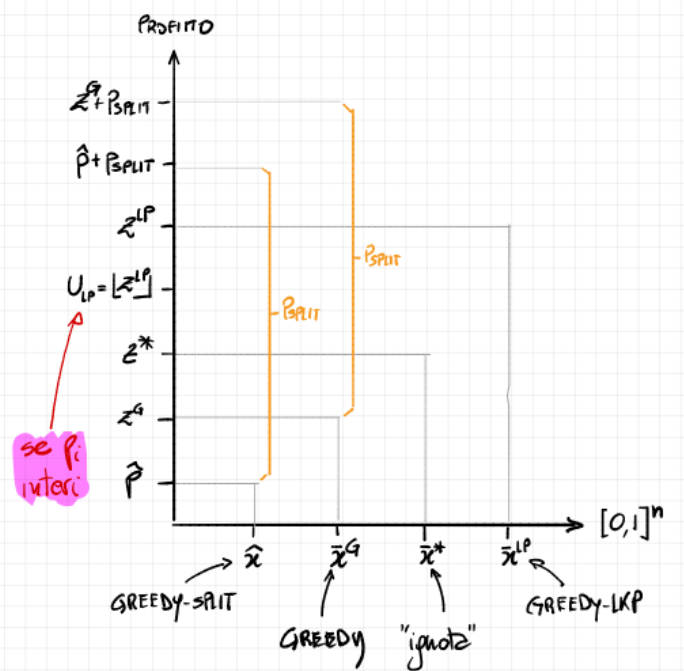
\includegraphics[width=0.6\textwidth]{./img/C_13.png}
\caption{Grafico della gerarchia di inclusioni} \label{FIG:C_13}
\end{figure*}\\
\subsection{C.14}
Nella creazione di un algoritmo \textit{Branch\&Bound} per \emph{KP} la prima cosa da fare è stabilire una \textbf{funzione costo}.Questo può essere fatto basandosi sulla gerarchia dei profitti degli algoritmi greedy vista in precedenza.In particolare il costo ad un \textit{E-node}$x[0..j)$ può essere scritto come:
$$\hat{c}(x[0..j)) = f(h(x[0..j))) + \hat{g}(x[0..j))$$
\begin{itemize}
	\item Nella prima parte dell'equazione abbiamo il \textit{costo noto}, che non è altro che la somma di tutti i profitti dei nodi "inseriti nello zaino" fin'ora ed i loro pesi. 
		\begin{equation}
                	f(h(x[0..j))\begin{cases}
			fh.w(x[0..j))= \sum_{0\leq k < j} x_{k}w_{k}\\
			fh.z(x[0..j))= \sum_{0\leq k < j} x_{k}p_{k}\notag
                \end{cases}
	        \end{equation}
	\item La seconda parte di equazione fornisce una stima per eccesso del profitto ottenibile (\textit{Upper bound}).
		\begin{equation}
			\hat{g}(x[0..j))\begin{cases}
				\hat{g}.w(x[0..j))= (\sum_{j\leq k < split} w_{k})+(c-[fh.w(x[0..j)) + \sum_{j\leq k < split} w_{k}]\\
				\hat{g}.z(x[0..j))= (\sum_{j\leq k < split} p_{k})+(c-[fh.w(x[0..j)) + \frac{\sum_{j\leq k < split} w_{k}]}{W_{split}}P_{split} \notag
                	\end{cases}
	        \end{equation}
	\item Una terza misura utile a scrivere un algoritmo \textit{Branch\&Bound} per il problema Knapspack è una stima per difetto (\textit{Lower Bound}), facilmente ottenibile tramite l'algoritmo greedy (o greedy split).
		\begin{align}
				z^g(x[0..j)) &= \sum_{0\leq k < j} x_{k}p_{k} + \sum_{j\leq k < split} p_{k} + \sum_{split < k < n} x_{k}p_{k} \notag \\
			&se \sum_{0\leq k < j} x_{k}w_{k} + \sum_{j\leq k < split} w_{k} + \sum_{split < k < n} x_{k}w_{k}\notag
		\end{align}
\end{itemize}
Una volta descritte le 3 misure si può impostare un algoritmo per la risoluzione \textit{Branch\&Bound} che rispetti la seguente invariante: In qualsiasi istante della visita $lower \; bound < z^* < upper \; bound$\\
L'idea di base è quindi quella di raffinare tramite le diverse iterazioni i due limiti fino ad ottenere la miglior \emph{soluzione} che sarà la \emph{risposta}.\\
\textit{Passo base}:
\begin{adjustwidth}{.8cm}{0cm}
		Non avendo visitato alcun nodo l' \textit{E-node} è la radice dello spazio degli stati.
		Il \textit{lower bound} è quindi l'algoritmo greedy scelto applicato al problema completo, allo stesso modo l' \textit{upper bound} è il risultato dell'algoritmo di soluzione di \emph{LKP} applicato al problema completo.
		In questo stadio la miglior soluzione (che identifichiamo come $x[0..r)$) è la soluzione trovata tramite l'algoritmo greedy.
\begin{figure*}[!ht]
\centering
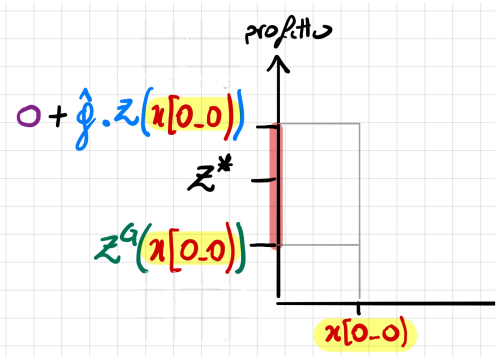
\includegraphics[width=0.7\textwidth]{./img/C14_profitto_z.png}
\caption{Bounds del profitto z} \label{FIG:C14_profitto_z}
\end{figure*}\\
\end{adjustwidth}
\textit{Passo induttivo}:
\begin{adjustwidth}{.8cm}{0cm}
	Al passo induttivo l'attuale \textit{E-node} sarà $x[0..j)$ e il nodo che fornisce la miglior soluzione $x[0..r)$ garantisce un profitto $z^*(x[0..r))$.
	Durante la visita dell' \textit{E-node} si possono presentare 4 situazioni (non esclusive):
	\begin{itemize}
		\item $f(h(x[0..j)) > C$\\
			Non ha senso "espandere" il nodo e proseguire nella visita del sotto-albero $T[0..j)$ in quanto sicuramente non otterremo una risposta avendo superato la capacità massima.Il nodo viene etichettato come \textbf{"completo"}, si sta effettuando \textit{pruning}.
		\item$f(h(x[0..j)) + \hat{g}.z(x[0..j)) < z^*(x[0..r))$\\
			Il profitto ottenibile espandendo il nodo è < dell'approssimazione per difetto trovata in uno dei passi precendenti.Anche inserendo tutti gli oggetti fino a capienza massima non si troverebbe una soluzione migliore di quella attuale (ricordo essere $z^*(x[0..r))$).Il nodo viene etichettato come \textbf{"completo"}, si sta effettuando \textit{pruning}.
\begin{figure*}[!ht]
\centering
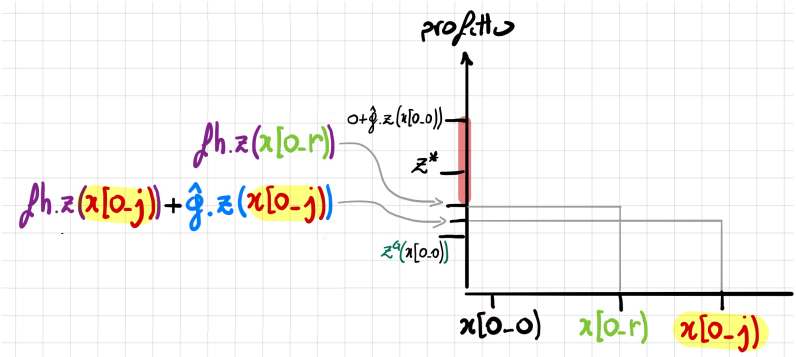
\includegraphics[width=0.7\textwidth]{./img/C14_item2.png}
\caption{nessun miglioramento rispetto alla soluzione del nodo $x[0..r)$} \label{FIG:C14_item2}
\end{figure*}\\
		\item $f(h(x[0..j)) < C \land f(h(x[0..j)) + \hat{g}.z(x[0..j)) > z^*(x[0..r))$\\
			Il sottoalbero $T[0..j)$ può ancora generare \textit{soluzioni}, fra queste potrebbe essere presente la \textit{risposta}.E quindi necessario \textbf{espandere} il nodo e continuare l'esplorazione del sottoalbero.
		\item $f(h(x[0..j)) < C \land f(h(x[0..j)) > z^*(x[0..r))$\\
			E' stata trovata una \textit{soluzione} che migliora il profitto $z^*(x[0..r))$, viene salvata ed i passi successivi faranno riferimento al profitto generato da $x[0..j)$.
	\end{itemize}
	\begin{figure*}[!ht]
\centering
\textbf{$((2,4,6,9),(10,10,12,18),15) \in KP$}
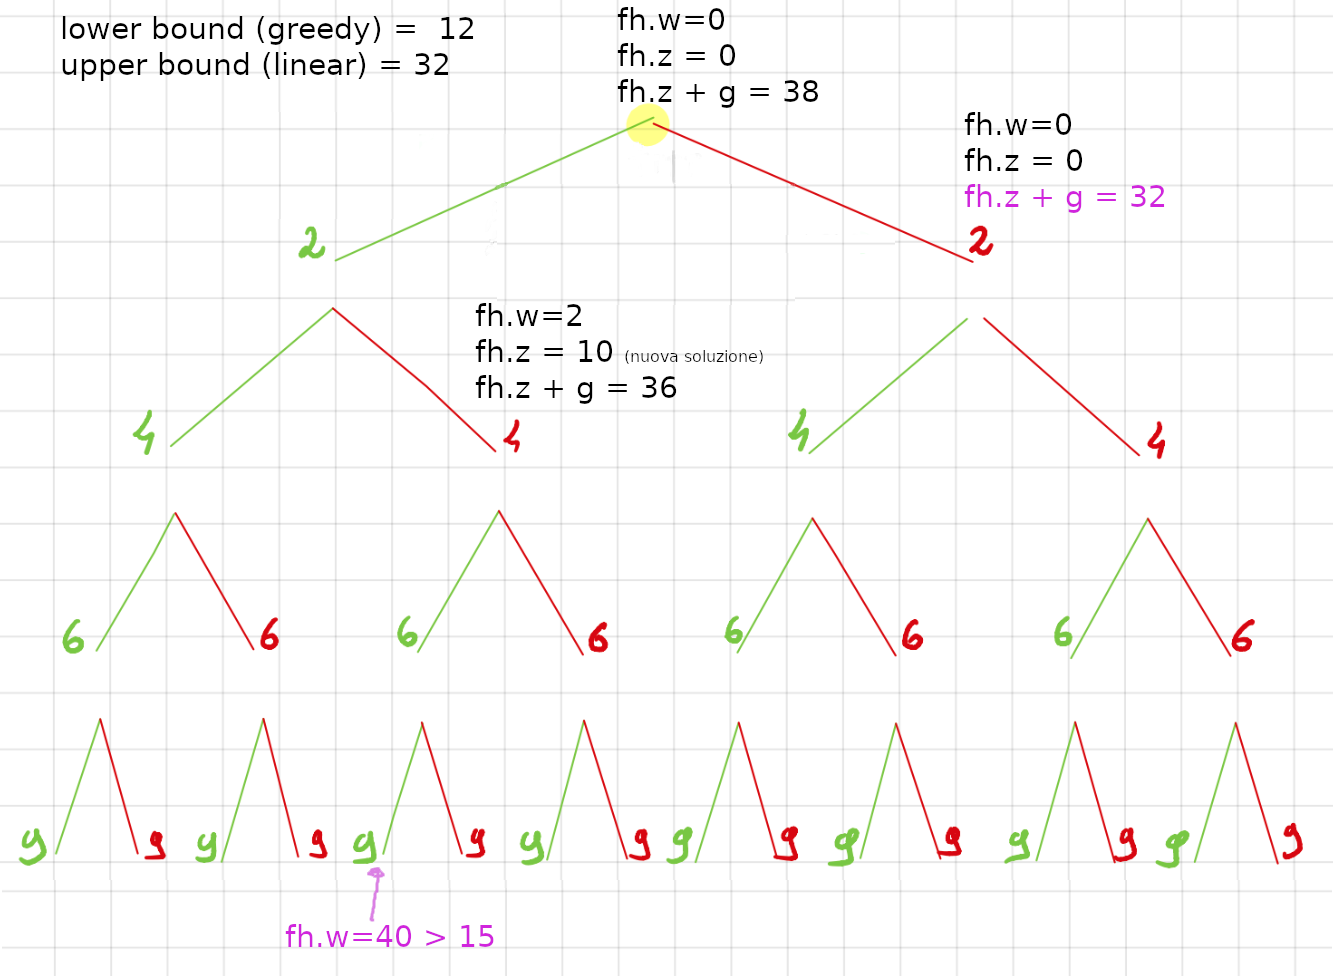
\includegraphics[width=1\textwidth]{./img/C14_BB_manuale.png}
\caption{Esempio di Branch\&Bound} \label{FIG:C14_BB_manuale}
\end{figure*}
	La cosa non specificata dall'algoritmo è il criterio di scelta del prossimo \textit{E-node} tra i vari \textit{live-nodes} disponibili.Utilizzando un criterio FIFO si ottengono buoni risultati, ma usando una tecnica \emph{least-cost} si è scoperto sperimentalmente che le prestazioni sono migliori.
	Intuitivamente ci sono due motivi per questo: in primis se $z^{LP} = Z^*$ è possibile che venga trovata una soluzione che sappiamo con certezza essere anche \textit{risposta}, si può quindi fare pruning dei restanti rami.
	In secondo luogo è possibile che giungendo "prima" alle \textit{soluzioni} migliori il valore di $z^*(x[0..r))$ cresca rapidamente causando il "rifiuto" di nodi che con una politica FIFO sarebbero stati espansi.(I nodi vengono rifiutati per la situazione 2)
\end{adjustwidth}
\section{Programmazione dinamica}
\subsection{D.1}
Il \textit{problema dello zaino} può essere suddifiso in una serie di sotto-problemi \textbf{KP} tra di loro indipendenti, prendiamo ad esempio $KP = (\vec w = (3,5,9,4), \vec p = (5, 6, 7, 3),9)$\\
Questo problema puù essere visto secondo il seguente formalismo:$$ max \sum_{j=1}^4 p_jx_j \text{ con } \sum_{j=1}^4 w_jx_j$$
Estraendo l'elemento di indice 4 si ottiene: $ max\; 3x_4 \sum_{j=1}^4 p_jx_j \text{ con } 4x_4\sum_{j=1}^4 w_jx_j$.
In tal modo si può generare l'albero delle scelte seguendo il formalismo, ad esempio la scelta $x=[?,1, 0 ,1]$ (scelta incompleta, non è una \textit{soluzione}) può essere formalizzata in:
$max\; 3 + 6 +5x_1 \sum_{j=1}^0 p_jx_j \text{ con } 4x_4\sum_{j=1}^4 w_jx_j$.\\
Sviluppando completamente l'albero delle scelte come in figura~\ref{FIG:D1_albero} si nota come l'istanza del problema \textbf{KP} presenta dei sottoproblemi condivisi, si può quindi configurare una soluzione che faccia uso delle tecniche di \textit{programmazione dinamica}.
\begin{figure*}[!ht]
\centering
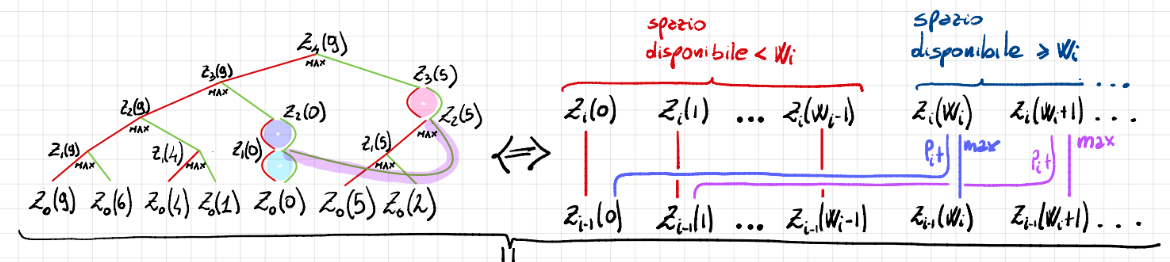
\includegraphics[width=1\textwidth]{./img/D1_albero}
\caption{Albero dei sottoproblemi} \label{FIG:D1_albero}
\end{figure*}\\
Volendo inserire l'elemento i-esimo abbiamo due possibili situazioni:
\begin{itemize}
	\item$W_i >$ spazio disponibile.Quindi $w_i$ non ci sta, la soluzione è identica alla soluzione del problema avente stesso spazio disponibile ma senza $w_i$.
	\item$W_i <$ spazio disponibile.In questo caso posso inserire $w_i$, ed il profitto generato sarà il massimo tra: la soluzione del problema senza $w_i$ e con spazio residuo "spazio disponibile - $w_i$ + il profitto generato da $i$ e la soluzione del problema senza $w_i$ con spazio residuo "spazio disponibile"
		Scritto in maniera più chiara e più formale: $$Z_i(W_i + sd)= \text{ max } \{ Z_{i-1}(sd - w_i) + P_i , Z_{i-1}(sd) \}$$ dove $sd$ è lo spazio disponibile.
		Intuitivamente nel primo caso abbiamo inserito nello zaino $i$ quindi il profitto è aumentato di $p_i$ e la dimensione diminuita di $w_i$, nel secondo caso non lo abbiamo aggiunto, quindi la soluzione ha lo stesso profitto della soluzione precedente.
\end{itemize}
Le due situazioni possono essere riassunte e formalizzate in questa formula ricorsiva:
\begin{equation*}
	z_j(sd)= \begin{cases} z_{j-1}(sd)\\ 
	\text{ max } \{ Z_{i-1}(sd - w_j) + P_j , Z_{j-1}(sd) \}
\end{cases}
\end{equation*}
Seguendo questa definizione ricorsiva si può ricavare un algoritmo che genera una "tabella dei profitti" completa.

Verrebbe da dire che la complessità di questo algoritmo è $O(n*c)$, ma la complessità va rapportata alla rappresentazione più efficiente dell'input.
Rispetto alla dimensione dell'input composto dai pesi $w_1, ..., w_n$ e dei profitti $w_1, ... , w_n$ ($| \vec w | = | \vec p | = n)$ la complessità è polinomiale.Il singolo peso (o profitto) è rappresentato tramite una notazione posizionale (probabilmente binario) e ci vogliono $n$ istanze di quella notazione per rappresentare tutti i pesi (o profitti).\\
Per $c$ la complessità non è polinomiale però. $c$ è un numero, ed in quanto numero è rappresentato da $2^b$ bit (presuppongo rappresentazione binaria).
Quindi al crescere di $c$ la sua rappresentazione cresce seguendo l'equazione $bits = 2^{1 + \lfloor \log_2c \rfloor}$ e ciò fa si che la complessità sia esponenziale rispetto a $c$.

La complessità dell'algoritmo di \textit{programmazione dinamica} per la risoluzione di \textbf{KP} è \imp{Pseudo polinomiale} in quanto è polinomiale per almeno uno dei valori dell'input ($c$).

\subsection{D.2}
L'algoritmo ricorsivo sviluppato tramite \textit{programmazione dinamica}permette di costruire una soluzione generando una tabella la cui ispirazione può essere ricondotta alla figura~\ref{FIG:D1_albero}.\\
\begin{center}
	\begin{tabular}{| c | c | c | c |}
  \hline
  $Z_n(0)$ & $Z_n(1)$ & ... &  $Z_n(c)$ \\
  \hline
  $ \vdots$ & $\vdots$ & $\vdots$ &  $\vdots $ \\
  \hline
  $Z_1(0)$ & $Z_1(1)$ & ... &  $Z_0(c)$ \\
  \hline
  $Z_0(0)$ & $Z_0(1)$ & ... &  $Z_0(c)$ \\
  \hline
	\end{tabular}
\end{center}
Dall'idea di questa tabella il più semplice algoritmo iterativo che ne deriva è:
\begin{lstlisting}[numbers=left,firstnumber=1,stepnumber=1, xleftmargin=15pt, language=Matlab ]
for d = 0 to c
    z[0][d] = 0
for j = 1 to n do
    for d = 0 to w[j] -1 do
    	z[j][d] = z[j-1][d]
    for d = w[j] to c do
	if z[j-1][d-w[j]] + p[j] > z[j-1][d] 
	    z[j][d]=z[j-1][d-w[j]] + p[j]
	    A[j][d]=1
	else
	    z[j][d] = z[j-1][d]
	    A[j][d]=0
z_sol=z[n][c]
\end{lstlisting}
\begin{itemize}
	\item nelle righe 1-2 vi è l'inizializzazione, la prima colonna $z_0(0),...,z_n(0)$ è impostata a 0 dato che non c'è spazio nello zaino per inserire nessun elemento.\\
	\item Le righe 4-5 illustrano la situazione "$j$ è troppo grande per essere inserito", quindi viene copiato il valore del passo precedente
	\item Dalla riga 6 alla riga 12 abbiamo l'implementazione dell'eq ricorsiva
	\begin{equation*}
        	z_j(sd)= \begin{cases} z_{j-1}(sd)\\
        	\text{ max } \{ Z_{j-1}(sd - w_j) + P_i , Z_{j-1}(sd) \}
	\end{cases}
	\end{equation*}
	Nelle righe 7-9 abbiamo il caso in cui $j$ migliora la soluzione, quindi la soluzione viene aggiornata aggiungendo $j$, nelle righe 11-12 invece abbiamo la situazione in cui è meglio mantere la vecchia soluzione dato che questa fornisce un profito migliore.
\end{itemize}
IMMAGINE TABELLA SU CUI FARE L'ESEMPIO QUANDO IL PROF LA CARICA
Questo algoritmo si porta dietro una struttura dati aggiuntiva, la tabella $A$ che mantiene l'informazione di quale sia la tupla che risolve il problema (la \textit{risposta}).

Una prima ottimizzazione sullo spazio si può fare liberandosi di questa matrice e ricavando la tupla \textit{risposta} dalla tabella $z$.\\
\begin{figure*}[!ht]
\centering
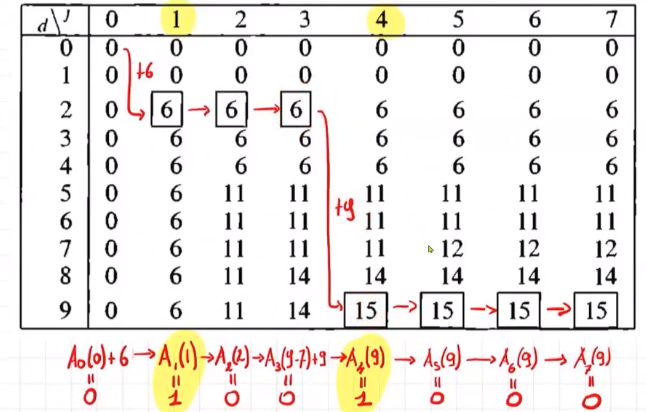
\includegraphics[width=1\textwidth]{./img/D2_ricavo}
\caption{Ricostruzione della tupla risolvente} \label{FIG:D2_ricavo}
\end{figure*}\\
Partendo dal valore $z_n(c)$ si ripercorre "all'indietro" l'algoritmo, se non vi è una variazione di valore è perchè si è preso il secondo ramo dell'if (riga 10), se vi è una variazione è perchè e stato aggiunto un elemento allo zaino.Bisogna quindi individuare la colonna in cui tale variazione è avvenuta e segnarsi l'indice della stessa (dato che gli indici delle colonne corrispondono agli indice del vettore di elementi $x$).\\
Ma come ricavare $z_{j-1}(d)$ in modo da sapere con quale "riga proseguire"? Basta rimuovere il profitto dell'elemento $j$ dalla cella $z_{j}(d)$ per individuare quale fosse il valore prima dell'aggiunta, cercare il valore corrispondente sulla $j-1$.
% il disegno andrebbe cambiato. si parte da z_n(c)

Si può ottimizzare ancora andando a "ridurre" la tabella a due soli array, uno contenente i valori della $i-1$-esima colonna e l'altro contenente i valori della colonna con indice $i$, attualmente in costruzione.\\
Una volta completato il calcolo della colonna $i$ questa diventerà la colonna $i-1$ e verrà usata per generare la colonna successiva, fino alla colonna $c$.\\
Ma si può ancora proseguire accorpando i due vettori, infatti non è necessario mantenere l'informazione delle celle che non cambiano valore.Basta calcolare i nuovi valori usando i valori scritti nel resto del vettore avendo cura di aggiornare il vettore partendo "dal fondo".\\
Le due ottimizzazioni sono rappresentate in figura~\ref{FIG:D2_ottimizzazioni}, e notiamo che effettuandole si perde però la possibilità di ricavarsi la tupla soluzione $x$ partendo dalla tabella.
Notiamo anche che tutte queste ottimizzazioni sono relative alla memoria, non al tempo, che resta sempre $O(n*c)$
\begin{figure*}[!ht]
\centering
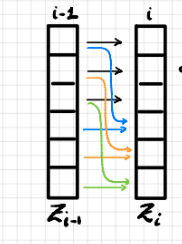
\includegraphics[width=0.4\textwidth]{./img/D2_2vettori}
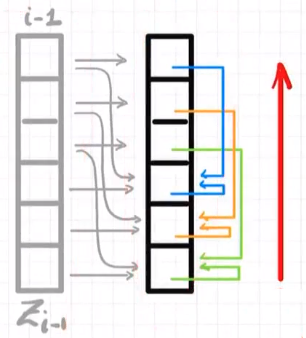
\includegraphics[width=0.4\textwidth,height=0.32\textheight]{./img/D2_1vettore}
\caption{Ottimizzazioni della tabella} \label{FIG:D2_ottimizzazioni}
\end{figure*}\\

\section{Complessità computazionale}
\subsection{E.1}
Una volta accordatici su una ragionevole rappresentazione dell'input si può parlare dei modelli di computazione, riconducendoci alla capacità degli automi (Macchine di Turing) di riconoscere un linguaggio.\\
Le Macchine di Turing deterministiche (\textbf{DTM}) sono composte da un nastro infinito ed una testina in grado di leggere e scrivere, in particolare hanno 3 caratteristiche:
\begin{enumerate}
	\item un set finito di simboli scrivibili sul nastro (alfabeto).
	\item un set di stati in cui sono presenti alcuni stati particolari: uno \textit{stato iniziale} ed uno o più \textit{stati finali}.
	\item una fuzione di transizione che deterministicamente spiega come si muove la testina.Deterministicamente poichè dato uno stato ed un simbolo in input segue una sola possibile configurazione futura.
\end{enumerate}
Posta una \textbf{DTM} si può informalmente definite la complessità come \textit{il numero di "passi" necessari alla computazione prima di giungere in uno stato finale}, naturalmente in realazione alla lunghezza dell'input.\\
La classe \textbf{PTime} contiene tutti i problemi che possono essere risolti tramite una \textbf{DTM} in un numero di "passi" polinomiale.Formalmente: $$\exists p \; t.c. \; \forall x \in \{0,1\}^* \; costo(DTM(x)) \leq p(\lvert x \rvert)$$
Cioè esiste un polinomio $p$ tale che per ogni possibile sequenza di 0 ed 1 in input ha un costo computazionale minore o uguale del calcolo del polinomio sulla dimensione della sequenza di input.
\begin{figure*}[!ht]
\centering
\includegraphics[scale = 0.5]{./img/E1_DTM.png}
\caption{costo di DTM(x)} \label{FIG:E1_DTM}
\end{figure*}


La classe \textbf{NPTime} si basa invece sul concetto di Macchina di Turing \textbf{non} deterministica (\textbf{NDTM}).\\
A differenza delle \textbf{DTM} non vi è una sola "testina", bensì due: un \textit{controllo a stati finiti} che può leggere o scrivere (è la testina della \textbf{DTM}), limitato a lavorare sulle celle$[0 + \infty)$, ed un \textit{guessing module} che lavora invece sulle celle $[-1,- \infty)$.\\
Questo "oracolo" scrive a caso nelle celle, generando una sequenza casuale di simboli dell'alfabeto (\textit{guessing stage}.
Anche la lunghezza della stringa generata è casuale, potenzialmente infinita.\\
Una volta concluso il lavoro del \textit{guessing module} il \textit{controllo a stati finiti} inizia a computare non solo basandosi sull'input e sullo stato, ma anche sulla stringa generata dall' \textit{oracolo} in maniera non predicibile \textit{checking stage}.
Una stringa è accettata se il \textit{controllo a stati finiti} si ferma su uno stato di accettazione, per una qualche stringa generata dal \textit{guessing module}, se non vi è alcuna stringa "oracolare" che permette di arrivare ad uno stato di accettazione la stringa è rifiutata.
%vedila come una computazione parallela. il guessing module rappresenta tutto il possibile spazio degli stati


La classe \textbf{NPTime} contiene tutti i problemi che possono essere risolti tramite una \textbf{NDTM} in un numero di "passi" polinomiale.Formalmente: $$\exists p \; t.c. \; \forall x \in \{0,1\}^* \; costo(NDTM(x)) \leq p(\lvert x \rvert)$$
È possibile vedere questa classe di algoritmi anche sfruttando il formalismo delle \textbf{DTM}
$$\exists p \; t.c. \; \forall x \in \{0,1\}^* \; costo(DTM(x,y)) \leq p(\lvert x \rvert)$$
	Cioè la sequenza in input viene verificata in tempo polinomiale rispetto alla dimensione dell'input da una \textbf{DTM} a cui viene fornita non solo l'input ma anche la stringa generata dall'oracolo che si sà condurre ad una soluzione (comunenmente detta certificato).
\begin{figure*}[!ht]
\centering
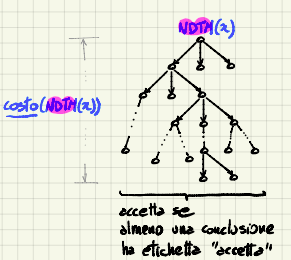
\includegraphics[scale = 0.5]{./img/E1_NDTM.png}
\caption{costo di NDTM(x)} \label{FIG:E1_NDTM}
\end{figure*} 
\subsection{E.2}
Utlizzare il formalismo delle macchine di Turing è scomodo e complesso per essere usato direttamente per il calcolo del costo computazionale.
Abbiamo bisogno di lavorare su strutture dati complesse con strumenti più "di alto livello" senza doverci per forza ricondurre al binario, ma mantenendo la possibilità di definire la complessità.\\
La soluzione è definire dei linguaggi in cui poter scrivere i programmi che corrispondano ad una macchina di Turing, semplificandone l'utilizzo, come se fosse una API per interagire con una macchina di Turing.
\begin{itemize}
	\item LID (\textit{Linguaggio Imperativo Deterministico}) corrispondente alle \textbf{DTM}\\
		Possiamo quindi dire che la classe \textbf{PTime} è l' insieme dei problemi risolvibili da programmi scritti in un linguaggio imperativo, deterministico .\\
		%(in un numero di passi polinomiale?)
		Questo linguaggio è la base di ogni linguaggio di programmazione, dato che fornisce le operazioni di:
		\begin{itemize}
			\item assegnazione: la possibilità di assegnare a variabili valori calcolati con espressioni aritmetiche.
			\item sequenza: possibilità di decidere in che ordine verranno eseguite le assegnazioni
			\item selezione: decidere in funzione del valore di una variabile quale operazione eseguire
			\item iterazione: ripetere più volte una operazione.
		\end{itemize}
	\item LNID (\textit{Linguaggio Non Imperativo Deterministico}) corrispondente alle \textbf{NDTM}\\
		Questo linguaggio estende il LID aggiungendo una operazione \textit{scelta(n)}.
		Questa primitiva genera $n$ "branch" paralleli che proseguono l'esecuzione.\\
		Ad esempio l'istruzione \texttt{x <- scelta(3)} produce 3 "thread" che eseguono la prossima istruzione uno usando $x=0$, un altro usando $x=1$ e l'ultimo usando $x=2$.\\
		\begin{figure*}[!ht]
		\centering
		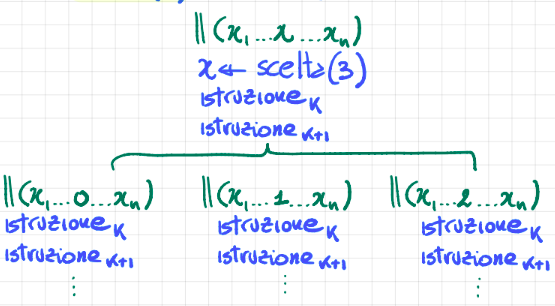
\includegraphics[scale = 0.5]{./img/E2.png}
		\caption{Istruzione scelta} \label{FIG:E2}
		\end{figure*}\\
		In tal modo è possibile generare una programma che contemporaneamente computa tutti it possibili stati dell'albero delle scelte, come mostrato in figura~\ref{FIG:E1_NDTM}
		\end{itemize}
\subsection{E.3}
Utlizzare il formalismo delle macchine di Turing è scomodo e complesso per essere usato direttamente per il calcolo del costo computazionale.
Abbiamo bisogno di lavorare su strutture dati complesse con strumenti più "di alto livello" senza doverci per forza ricondurre al binario, ma mantenendo la possibilità di definire la complessità.\\
La soluzione è definire dei linguaggi in cui poter scrivere i programmi che corrispondano ad una macchina di Turing, semplificandone l'utilizzo, come se fosse una API per interagire con una macchina di Turing.

È possibile basare la definizione di classe \textbf{PTime} su un linguaggio \textbf{LID} (e quella di \textbf{NPTime} su un linguaggio \textbf{LIND}) perchè esiste una codifica tra il linguaggio e la macchina che non introduce complessità computazionale maggiore di un polinomio.
Cioè è possibile "simulare" il funzionamento dell'algoritmo tramite una macchina di Turing e il costo di questa \textit{simulazione} è polinomiale.\\
La figura~\ref{FIG:E3} mostra che è possibile simulare un passo di un algoritmo, scritto in un linguaggio, facendo compiere una serie di passi ad una macchina di Turing.Posto di voler simulare $c$ passi dell'algoritmo la corrispondente macchina necessiterà di $s(c)$ passi, ove la funzione $s$ è polinomiale.
Perciò possiamo affermare che un algoritmo scritto in linguaggio \textbf{LID} ha una data complessità perchè è possibile simulare il suo funzionamento tramite una macchina di Turing inserendo un overhead al massimo polinomiale, quindi senza modificare la sua complessità.
\begin{figure*}[!ht]
\centering
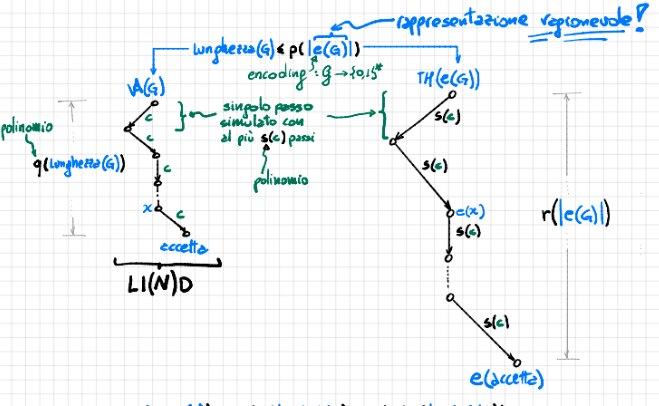
\includegraphics[width = 1\textwidth]{./img/E3.png}
\caption{Overhead polinomiale} \label{FIG:E3}
\end{figure*}\\

\subsection{E.4}
n
La teoria della \imp{NP-completeness} si è sviluppata in relazione alla complessità di problemi decisionali, non di ottimizzazione, a causa di come si è evoluta la teoria degli automi.\\
Infatti utilizzando il formalismo degli automi (Macchine di Turing) risulta molto più naturale guardare al problema come se fosse un linguaggio da decidere. Se l'input fornito appartiene al linguaggio l'automa risponderà \textit{True}, \textit{False} altrimenti.\\
Nasce quindi la necessità di passare da problemi di ottimizzazione a problemi decisionali, per poterne valutare la complessità, e viceversa.

Analizziamo il caso del problema \textbf{KP} per spiegare informalmente che questa trasformazione è sempre possibile.
\begin{itemize}
	\item Ottimizzazione $\rightarrow$ Decisione, risolvere il problema decisionale vuol dire risolvere anche il corrispettivo problema di ottimizzazione.\\
	Dato un algoritmo che risolve \textbf{KP(l,c)} possiamo costruire un algoritmo per risolvere \textbf{KP(c)}, l'intuizione è sollevare il \textit{lower bound l} finchè non trovo più alcuna soluzione.
Segue l'algoritmo in pseudocodice in cui l'operazione $sum(p\_i)$ indica la somma di tutti i pesi degli elementi del vettore soluzione trovato.
\begin{lstlisting}[xleftmargin=15pt, language=Java ]
l=0
z*=0
for (l=0 ; l <= sum(p_i), l++)
    if(KP(l,c) != true)
        z* = l-1
return z*
\end{lstlisting}
\item Decisione $\rightarrow$ Ottimizzazione, risolvere il problema di ottimizzazione vuol dire risolvere anche il corrispettivo problema decisionale.\\
	Nel caso del problema \textbf{Knapsack} è molto semplice da dimostrare.Avendo un algoritmo che risolve \textbf{KP(c)} possiamo ottenere una soluzione $z^*$, se tale soluzione è $\leq l$ rispondiamo $True$ al problema decisionale, $False$ altrimenti:

\begin{lstlisting}[xleftmargin=15pt, language=Java ]
z* = KP(c)
if (z >= l)
    return true
else
    return false
\end{lstlisting}
\end{itemize}
\subsection{E.5}
La \textit{riduzione} tra problemi decisionali è un'operazione che permette di confrontare due problemi computazionali e la complessità delle loro soluzioni.\\
Si indica con "$\leq_p$", quindi $P_1 \leq_p P_2$ significa affermare che se $P_2$ si può risolvere "velocemente" allora anche $P_1$ può essere risolto velocemente.
Negando l'implicazione se non è noto alcun algoritmo polinomiale per risolvere $P_2$ nemmeno $P_1$ può essere risolto in tempo polinomiale.
Formalmente:
\begin{definition}[Riduzione]
	Dati $P_1$ e $P_2$ problemi computazionali. $P_1 \red P_2$ se $\exists F: Dom(P_1) \rightarrow Dom(P_2)$ con le seguenti proprietà:
	\begin{itemize}
		\item se $x \in Dom(P_3) \text{ ed } x \; istanza \; di \; P_1 \Rightarrow F(x) \; istanza \; di \; P_2$, cioè se l'algoritmo che risolve il problema decisionale $P_1$ ritorna \textit{vero} quando viene data in input l'istanza $x$ allora ritornerà \textit{vero} l'algoritmo che risolve $P_2$ data in input l'istanza $F(x)$.
		\item se $x \in Dom(P_1) \text{ ed } x \text{ non è istanza di }P_1 \Rightarrow F(x) \; istanza \; di \; P_2$, cioè se l'algoritmo che risolve il problema decisionale $P_1$ ritorna \textit{falso} quando viene data in input l'istanza $x$ allora ritornerà \textit{falso} l'algoritmo che risolve $P_2$ data in input l'istanza $F(x)$.
		\item $\exists p, \forall x \; t.c. \; costo(Alg_F(x))\leq p(\lvert x \rvert)$, cioè il costo di applicare la trasformazione $F$ all'istanza $x$ è inferiore ad un polinomio calcolato sulla dimensione di $x$.
	\end{itemize}
\end{definition}
Posto \textbf{SAT} intrattabile si può affermare che \textbf{KP} è intrattabile perchè $SAT \red KP$, dalla seguente catena di riduzioni:
$$ SAT \red NNF \red CNF \red 3CNF \red 3COL \red EXCO \red Subsetsum KP$$
\begin{itemize}
	\item \textbf{SAT}: data una formula proposizionale $f$, dice se questa è soddisfacibile. $\exists \varphi \Phi _ {\varphi}(f) = true $
	\item \textbf{NNF}: data una formula Negation Normal Form $f$, dice se esiste una assegnazione delle variabili $FV(f)$ che soddisfa $f$.\\$\exists \varphi:FV(f) \in \{true,false\}^* \; t.c. \; \Phi _ {\varphi}(f) = true $
	\item \textbf{CNF}: data una formula $f$ scritta in Conjunctive Normal Form, dice se questa è soddisfacibile. $\exists \varphi \Phi _ {\varphi}(f) = true $.\\
$\exists \varphi:FV(f) \in \{true,false\}^* \; t.c. \; \Phi _ {\varphi}(f) = true $

\end{itemize}
PROSEGUIRE CON LE ALTRE
%PROSEGUIRE CON LE ALTRE
\subsection{E.6}
Le formule \textbf{NNF}(Negation Normal Form) sono tutte quelle formule in cui la negazione è presente solo sullevariabili, non sulle sotto-formule.
La sintassi diventa quindi:
$$ N ::= true|false|var|\overline{var}|N \land N|N \lor N$$
La \textit{funzione di riduzione} che permette di passare da formule proposozionali a NNF è ben conosciuta, solo le leggi di De Morgan:
$$ \overline{f \lor h} = \overline{f} \land \overline{h} \qquad \qquad \overline{f \land h} = \overline{f} \lor \overline{h}$$
L'intuizione è quella di "spingere" le negazioni presenti nella \textit{formula proposizionale} $f$ verso le variabili.
%cos'è "un qualche aspetto fondamentale"? tutta la dimostrazione?
DA FARE
\subsection{E.7}
Le formule in \textbf{CNF} (Conjunctive Normal Form) sono formule composte da una congiunzione di clausole a loro volta composte da una disgiunzione di letterali.
\begin{definition}[Sintassi]
	$$F::= [C]|[C],F \; congiunzione \: (\land)$$
	$$C::=true|false|l,C \; disgiunzione \: (\lor)$$
\end{definition}
Si può passare dalla forma in \textbf{NNF} alla forma in \textbf{CNF} grazie alla \textit{trasformazione di Tseytin}.\\
Intuitivamente l'idea è quella di somporre l'equazione in tutte le sue sottoparti, collegate tra loro da "collegamenti" che corrispondono alle equivalenze logiche.
Assegnando un nome ad ogni canale è possibile ricostruire la formula logica sotto forma di \textbf{NNF}, il modo più efficace di vedere questa equivalenza è un "circuito".
Analizzando ad esempio $[(\overline s \land p) \lor ((q \land \overline r) \land p)]$
\begin{figure*}[!ht]
\centering
\begin{forest}
	[$(\overline s \land p) \lor ((q \land \overline r) \land p)$[$\overline s \land p$, , edge label = {node[midway,left,red] {b}} [$\overline s$, , edge label = {node[midway,left,red] {d}}][$p$,, edge label = {node[midway,right,red] {e}}]][$((q \land \overline r) \land p)$, edge label = {node[midway,right,red] {c}} [$(q \land \overline r)$, edge label = {node[midway,left,red] {g}} [$q$, edge label = {node[midway,left,red] {f}}][$\overline r$, edge label = {node[midway,right,red] {h}}]] [$p$, edge label = {node[midway,right,red] {i}}]]]
\end{forest}
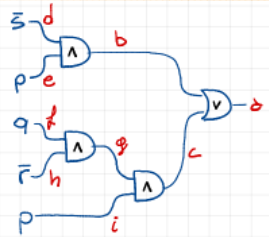
\includegraphics[width=0.4\textwidth]{./img/E7_circuit}
\caption{Trasformazione di Tseytin} \label{FIG:E7_circuit}
\end{figure*}\\
Ricomponendo si ottiene:
$$ a,(a \Leftrightarrow b \lor c), (b \Leftrightarrow d \land e), (c \Leftrightarrow g \land i), (g \Leftrightarrow f \land h)$$.
Eliminando le implicazioni si può ridurre la formula ad una formula avente solo congiunzioni (\textit{and}) fuori dalle parentesi e disgiunzioni (\textit{or}) dentro.
La trasformazione di \textit{Tseitin} può essere formalmente definita come:
\begin{definition}(Trasformazione di Tseitin)
 	Data $f$ funzione in Negation Normal Form, la trasformazione di Tseitin $T$ è:
	$$ T(f) = [a],C[a,f]$$
	Ove a è una nuova variabile, $C$ è una operazione del tipo $C: variabili \times NNF$
	$$C[a,l] = a \Leftrightarrow l$$
	$$C[a,f \circ g] = a \Leftrightarrow b \circ c, C[b,f],C[c,g]\; con \; \circ \in \{\land,\lor, \Rightarrow, \Leftrightarrow\}$$
	$b$ e $c$ nuove variabili.
\end{definition}
La \textit{Trasformazione di Tseitin} genera delle \textbf{CNF}, ma ciò va dimostrato:
\begin{theorem}[Correttezza trasformazione di Tseitin]
	$\forall f $ formula in \textbf{NNF} e $\forall a$ variabile $C(a,f) = c_1,...,c_n$ sono tutte clausole.
\end{theorem}
\begin{dimostrazione}
	Dimostrato per induzione su $f$, ci sono due possibilità:
	\begin{itemize}
		\item $f$ è un letterale $l$:
			\begin{equation*}
			C(a,l) = (a \Leftrightarrow l) = (a \Rightarrow l) \land (l \Rightarrow a)= 
			\text{ sostituendo l'implicazione } = [ \overline a, l],[ \overline l, a]
			\end{equation*}
			Cioè due clausole.
		\item $f = g \circ h$, cioè $f$ composizione di due operatori.
			\begin{align*}
				&C(a,l) = a \Leftrightarrow (b \circ c),C(b,g), C(c,h) \text{ per definizione della trasformazione} \\
				&a \Leftrightarrow (b \circ c), (C_1,...,C_n), (C_1',..., C_n') \text{ per ipotesi induttiva le due parentesi sono clausole}\\
				&= \text{ sostituendo le implicazioni } = \overline a \lor  (b \circ c), \overline{(b \circ c)} \lor a, (C_1,...,C_n), (C_1',..., C_n')
                        \end{align*}
			Tutte e quattro sono clausole.
	\end{itemize}
\end{dimostrazione}
\subsection{E:8}
La dimostrazione di $NNF \red CNF$ si basa su un lemma derivante dalla costruzione della \textit{funzione di Tseitin}
\begin{equation*}
	\text{Lemma T}\begin{cases}
		(\exists \varphi \Phi_\varphi(f) = true) \Leftrightarrow (\exists \varphi' \Phi_{\varphi'}(C[a,f]) = true \land \varphi'(a) = true)\\
		(\exists \varphi \Phi_\varphi(f) = false) \Leftrightarrow (\exists \varphi' \Phi_{\varphi'}(C[a,f]) = true \land \varphi'(a) = false)
	\end{cases}
\end{equation*}
\begin{theorem}
	$f \in NNF \Leftrightarrow T(f) \in CNF$ 
\end{theorem}
\begin{dimostrazione}
	Per definizione $T(f) = [a],C[a,f]$.
	\begin{itemize}
		\item se $f$ è soddisfacibile la sua trasformazione $T(f)$ è soddisfacibile, cioè $f \in NNF \Rightarrow \exists \varphi \Phi_\varphi(f) = true$\\
			Ci appoggiamo al Lemma T.1: 
			$$(\exists \varphi \Phi_\varphi(f) = true) \Leftrightarrow (\exists \varphi' \Phi_{\varphi'}(C[a,f]) = true \land \varphi'(a) = true)$$
			Cioè esiste se esiste una funzione $\varphi$ che assegna dei valori alle variabili di $f$ tali che rendono vera $\Phi(f)$ allora esiste un'altra funzione $\varphi'$ che applicata a $C[a,f]$ rende vera $\Phi(C[a,f]$ ed assegna il valore \textit{vero} alla nuova variabile $a$.$\varphi'$ è una "estensione" di $\varphi$ sulle nuove variabili generate da $C$ che comunque "rispetta" il comportamento di $\varphi$.\\
			Posto vero per ipotesi $\exists \varphi \Phi_\varphi(f)= true$ ho che $(\varphi'(a) \land \varphi' \Phi_{\varphi'}(C[a,f])i)=true$.\\
			Inserendo $\varphi'(a)$ come congiunzione all'interno della funzione di valutazione $\Phi_{\varphi'}$ si ottiene $\Phi_{\varphi'}([a],C[a,f])$ che riprendendo la definizione di $T$ è $\Phi_{\varphi'}(T(f))$.Quindi$\Phi_{\varphi'}(T(f))=true$, come volevasi dimostrare.
		\item se invece $f$ non è soddisfacibili la sua trasformazione $T(f)$ non deve essere soddisfacibile, cioè $f \notin NNF \Rightarrow \forall \varphi \Phi_\varphi(f) = false$\\
			Appoggiandosi al lemma T.2 abbiamo che
			$$(\exists \varphi \Phi_\varphi(f) = false) \Leftrightarrow (\exists \varphi' \Phi_{\varphi'}(C[a,f]) = true \land \varphi'(a) = false)$$
			Dato che abbiamo supposto per ipotesi $\forall \varphi \Phi_\varphi(f) = false$ allora $(\varphi'(a) \land \varphi' \Phi_{\varphi'}(C[a,f])i)=false$.\\
			Il Lemma T.2 ci suggerisce che il valore falso deriva dalla congiunzione $true \land false = false$.\\
			Come nel primo caso inserendo $\varphi'(a)$ come congiunzione all'interno della funzione di valutazione $\Phi_{\varphi'}$ si ottiene $\Phi_{\varphi'}([a],C[a,f])$.Cioè $\Phi_{\varphi'}(T(f)) = \Phi_{\varphi'}(T(f))=false$.\\
			La trasformazione genera una nuova variabile $a$ tale per cui $\varphi'(a) = false$ e tale variabile rende false tutta la valutazione $\Phi_{\varphi'}(\cdot)$.
	\end{itemize}
\end{dimostrazione}

\section{Problemi computazionali}
\subsection{F.1}
\begin{definition}[SubsetSum]
	Siano dati un insieme numerico finito $X$ ed un numero $S$. Determinare l’esistenza di un sottoinsieme $Y \subset X$, tale che la somma di tutti gli elementi di $Y$ sia pari ad $S$.
\end{definition}
	Vedendolo come problema decisionale può essere riscritto come:
	$$((w_1,...,w_n),S) \in SubsetSum \; se \; \exists x_1, ... , x_n \in \{0,1\}^n \: t.c. \sum_{1 \leq k \leq n} x_kw_k = S$$
	SubsetSum è un caso specifico di \imp{KP}, in particolare è un problema \textbf{Knapsack} in cui i profitti sono uguali ai pesi.
	$$((w_1,...,w_n),S) \in SubsetSum \Rightarrow ((w_1,...,w_n),(w_1,...,w_n),S) \in KP$$
\begin{dimostrazione}
	Per ipotesi $\exists x_1^., ..., x_n^. \: tc \sum_{j=1}^n w_jx_j = S$ cioè esiste una scelta di valori $x_1,...,x_n$ che risolve il problema. ($x_1^., ..., x_n^.$ è un istanza di $x_1, ..., x_n$)

	Dobbiamo dimostrare che esiste una soluzione del rispettivo problema \imp{KP} cioè che esista una istanza di scelte la cui somma dei pesi è minore di $S$ ma allo stesso tempo è la massima scelta possibile (è più grande del peso di ogni altra possibile istanza di scelte):
	$$ \exists z_1^., ..., z_n^. \: tc \forall y_1,...,y_n \sum_{j=1}^n w_jz_j \geq \sum_{j=1}^n w_jy_j \text{ e } \sum_{j=1}^n w_jz_j \leq S$$
	Prendendo come istanza $z^.$ l' istanza $z^.$ definita in precedenza abbiamo la sicurezza che, per ipotesi, $\sum_{j=1}^n w_jz_j \leq S$

	La tesi diventa quindi $$ \forall y_1,...,y_n \sum_{j=1}^n w_jx_j^. \geq \sum_{j=1}^n w_jy_j$$
Supponiamo per assurdo che esista una scelta che fornisce un peso maggiore di quello generato dall'istanza $x^.$:$$\exists y_1^.,...,y_n^. \sum_{j=1}^n w_jy_j^. > \sum_{j=1}^n w_jx_j^.$$
Allora $sum_{1 \leq j \leq n} w_jy_j^. > \sum_{j=1}^n w_jx_j^. = S $, ed essendo necessario identificare una sequenza di scelte $z_1,...,z_n$ t.c. $\sum_{j=1}^n w_jz_j \leq S$ non possiamo accettare $y^.$ come istanza risolutiva del problema dal momento che:
$$\sum_{j=1}^n w_jy_j^. > S $$
\end{dimostrazione}
\subsection{F.2}
Dimostrare che i problemi \emph{KP} e \emph{Bounded-KP} sono equivalenti.\\Cioè $KP \Leftrightarrow BKP$.\\
\begin{dimostrazione}
	$KP \Rightarrow BKP$: ogni problema \emph{KP} è un problema \emph{BKP}.\\
	La dimostrazione è immediata in quanto un generico problema\\$((P_1, ... ,P_n),(W_1, ... ,W_n),C)\in KP$ può essere riscritto come\\ $((P_1, ... ,P_n),(W_1, ... ,W_n),(1, ... ,1),C) \in BKP$.

	$KP \Leftarrow BKP$: ogni problema \emph{BKP} è un problema \emph{KP}.\\
	per prima cosa introduciamo $B_i + 1$ nuove variabili, $\forall i \in B_1 ... B_n$.\\
	Avremo quindi
	\begin{align}
		x_{0}', ... ,&x_{b_i}' \in \{0,1\}  \notag \\
   		&\;\;\vdots \notag \\
		x_{0}^n, ... ,&x_{b_i}^n \in \{0,1\}  \notag 
	\end{align}
	Queste variabili indicano "quanti" oggetti di tipo $x^i$ sto prendendo, quindi 
	\begin{equation}
		x_{j}^i=\begin{cases}
      		0\; se\; x_i = 0\\
      		1\; se\; x_i = j \notag
    		\end{cases}
	\end{equation}
	Il problema è diventato un esempio di \emph{BKP} di questo tipo:
	\begin{center}
		\scalebox{0.89}{$((p_1, 2p_1 ,...,b_1p_1, ... ,p_n, 2p_n, ..., b_np_n),(w_1, 2w_1 ,...,b_1p_1, ... ,w_n, 2w_n, ..., b_nw_n),C))$}\\
		$maximize \; \sum_{i=1}^{n} \sum_{j=0}^{b_i} p_j*j*x^i_j$\\
		$subject \; to \; \sum_{i=1}^{n} \sum_{j=0}^{b_i} w_j*j*x^i_j$\\
		con la condizione aggiuntiva $ \forall i \sum_{j=0}^{b_i} x_j^i = 1$
	\end{center}
	In modo che  si possano prendere solo $j$ oggetti fi tipo $x^i$
	%non posso prendere 5 x', e poi 3 x', sarebbe come prendere 8 x'
	DA FINIRE CON OSSERVAZIONE DEL PROF RIGUARDO AL FATTO DI DOVER DIMOSTRARE LA RISOLVIBILITà
\end{dimostrazione}
\end{document}
